% Figures for "On the Thermodynamic Consequences of Oscillatory Mechanics in Audio Processing"
% Conceptual figures (PDF) and experimental results (PNG)
% 
% PLACEMENT GUIDE:
% - Each figure includes section placement information
% - Insert figures in the specified sections of the main document
% - Maintain figure order within each section

% ========================================
% CONCEPTUAL FIGURES (PDF)
% ========================================

% SECTION: Problem Definition and Theoretical Foundation (Section 2.2)
\begin{figure}[htbp]
\centering
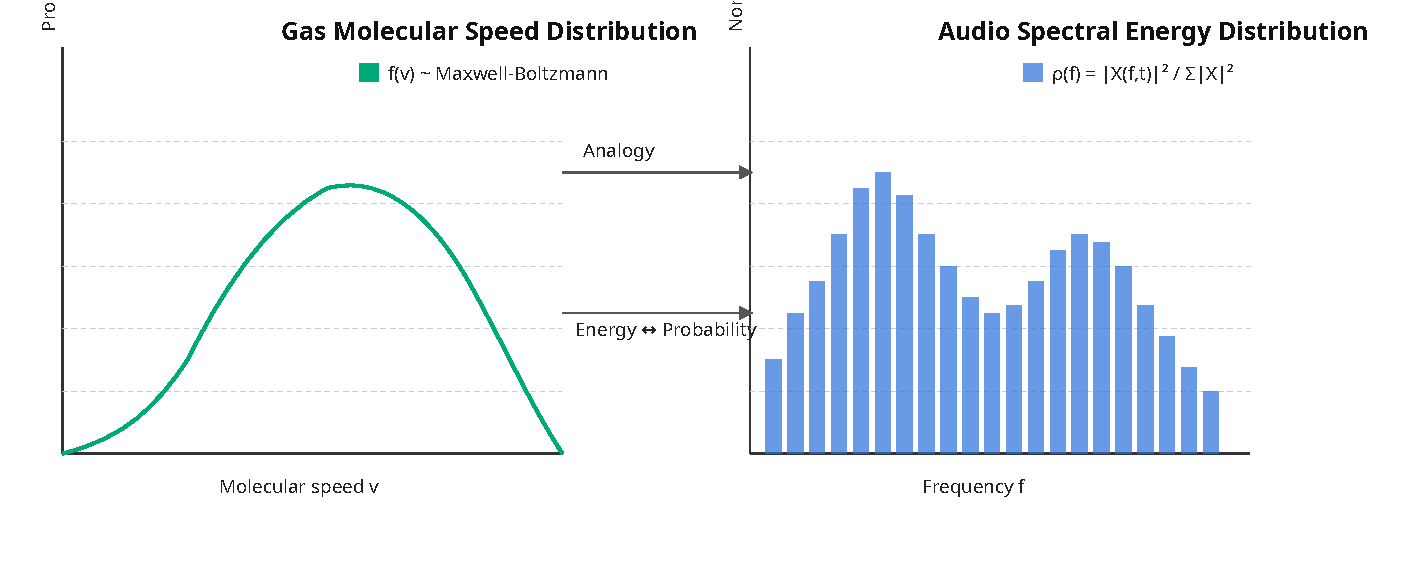
\includegraphics[width=0.9\textwidth]{images/gas_vs_audio.pdf}
\caption{Conceptual parallel between gas molecular distribution and audio spectral distribution. The normalized energy density $\rho(f,t)$ in the time-frequency domain exhibits properties consistent with molecular density distributions in statistical mechanics, providing the theoretical foundation for thermodynamic audio processing.}
\label{fig:gas_vs_audio}
\end{figure}

% SECTION: Problem Definition and Theoretical Foundation (Section 2.2)
\begin{figure}[htbp]
\centering
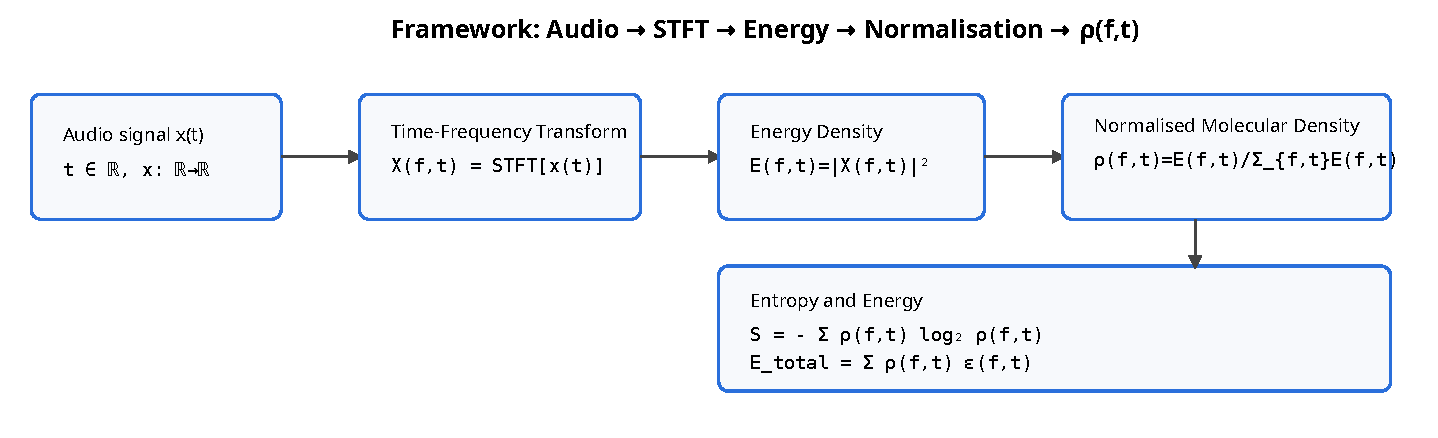
\includegraphics[width=0.85\textwidth]{images/mathematical_framework.pdf}
\caption{Mathematical framework progression from audio signal to gas molecular density distribution. The transformation sequence shows: (1) audio signal $x(t)$, (2) STFT representation $X(f,t)$, (3) normalized energy density $\rho(f,t)$, and (4) thermodynamic state variables including entropy $S$ and total energy $E_{\text{total}}$.}
\label{fig:mathematical_framework}
\end{figure}

% SECTION: Motivation - Transforming Neural Audio Processing (Section 1.2)
\begin{figure}[htbp]
\centering
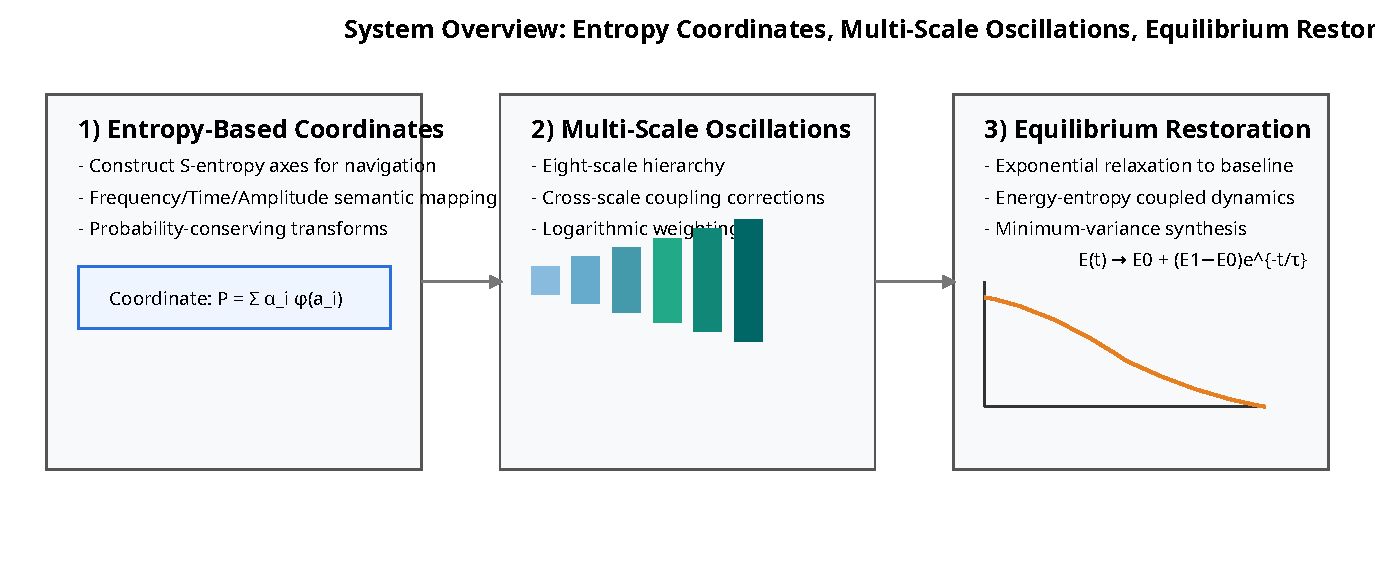
\includegraphics[width=0.9\textwidth]{images/system-components.pdf}
\caption{System architecture overview showing the three primary framework components: (1) S-entropy coordinate systems for audio space navigation, (2) multi-scale oscillatory analysis across hierarchical frequency ranges, and (3) thermodynamic equilibrium restoration for real-time meaning synthesis. The components work in concert to eliminate storage dependencies while maintaining computational efficiency.}
\label{fig:system_components}
\end{figure}

% SECTION: Oscillatory Foundation (Section 3.2)
\begin{figure}[htbp]
\centering
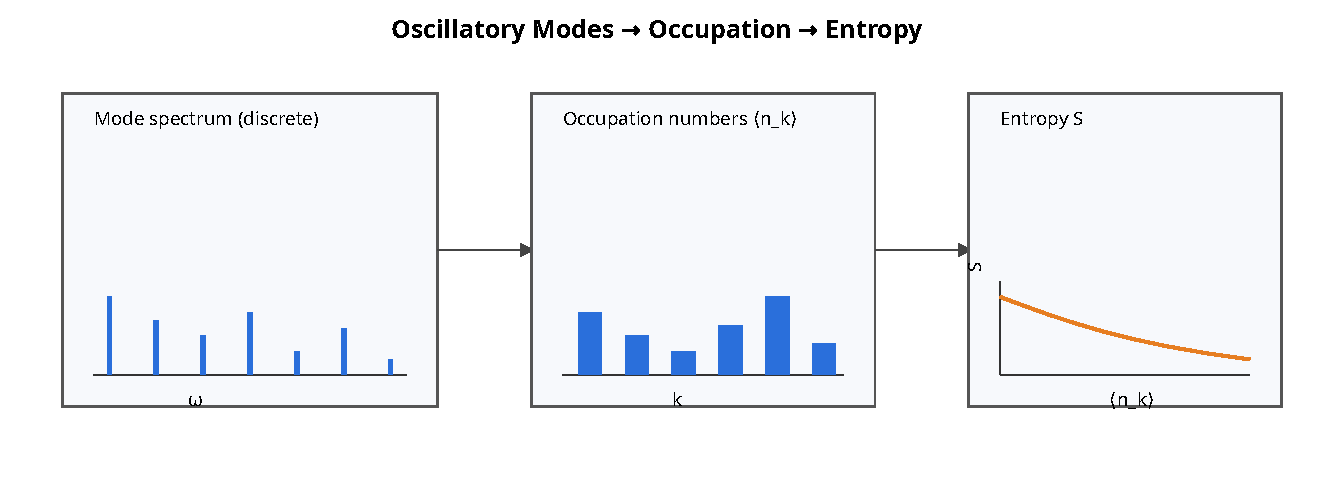
\includegraphics[width=0.8\textwidth]{images/oscillatory-mode.pdf}
\caption{Eight-scale oscillatory framework for hierarchical audio analysis. The framework spans from quantum acoustic signatures (10⁻¹⁵ Hz) to cultural dynamics (10⁻⁸ Hz), with electronic frequency analysis (40-20,000 Hz) serving as the primary scale for electronic music processing. Each scale contributes unique molecular information to the thermodynamic ensemble.}
\label{fig:oscillatory_modes}
\end{figure}

% SECTION: St-Stellas Framework Application for Audio Processing (Section 5.1)
\begin{figure}[htbp]
\centering
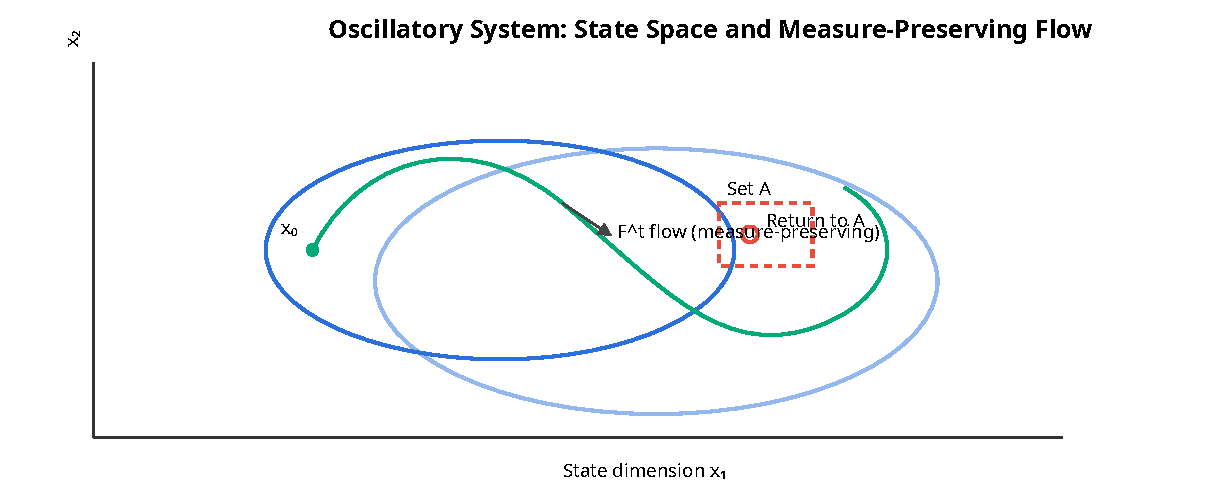
\includegraphics[width=0.85\textwidth]{images/oscillatory_state_transform.pdf}
\caption{St-Stellas coordinate transformation for audio elements. The cardinal direction mapping transforms rhythmic, harmonic, dynamic, and textural audio elements into geometric coordinates, enabling S-entropy navigation and cross-modal pattern recognition through the empty dictionary architecture.}
\label{fig:stellas_transform}
\end{figure}

% SECTION: Thermodynamic Models for Audio Processing (Section 4.2)
\begin{figure}[htbp]
\centering
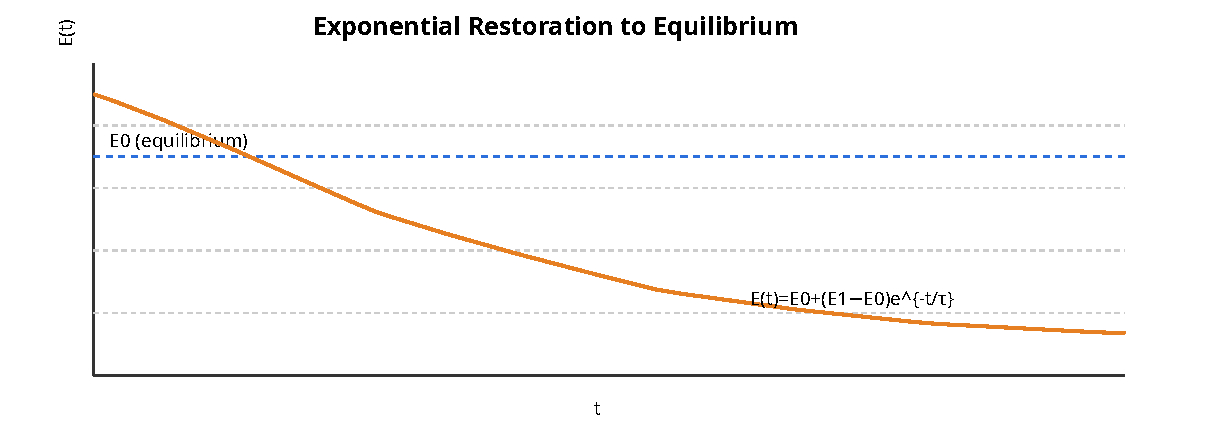
\includegraphics[width=0.9\textwidth]{images/time-series-restoration-dynamics.pdf}
\caption{Thermodynamic equilibrium restoration dynamics showing the pathway from acoustic perturbation to equilibrium state. The restoration process follows exponential decay with time constant $\tau$, demonstrating minimum variance synthesis as the system returns to baseline thermodynamic equilibrium through optimal energy pathways.}
\label{fig:restoration_dynamics}
\end{figure}

% SECTION: Thermodynamic Models for Audio Processing (Section 4.4)
\begin{figure}[htbp]
\centering
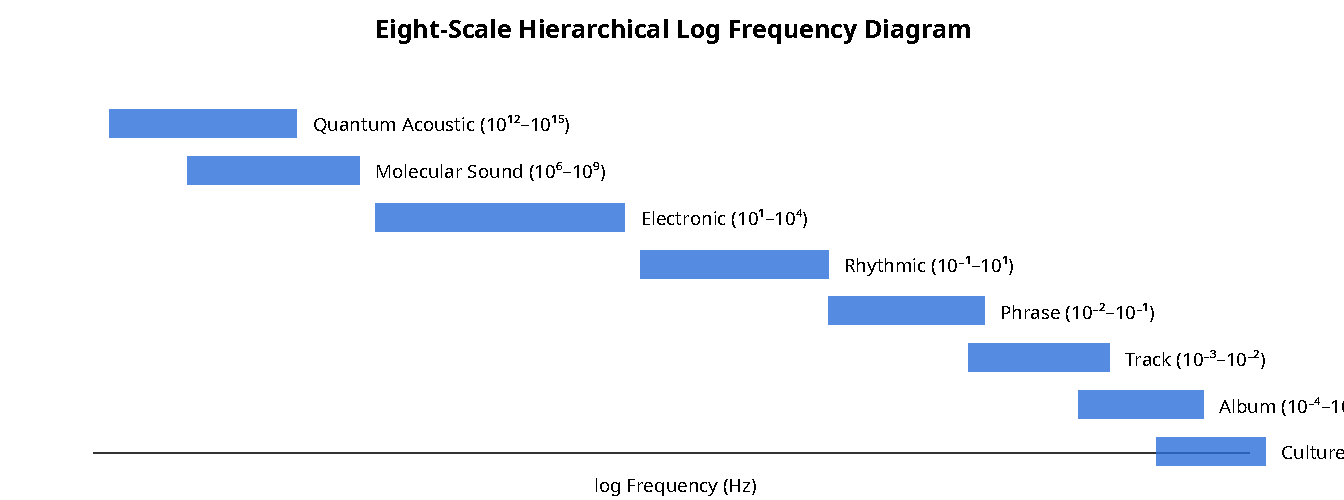
\includegraphics[width=0.8\textwidth]{images/logarithmic_frequency.pdf}
\caption{Logarithmic frequency band decomposition for electronic music analysis. The six-band structure (kick fundamental, bass synth, lead synth, pad sweep, hi-freq elements, air band) provides genre-specific energy distribution patterns while maintaining thermodynamic consistency across molecular ensembles.}
\label{fig:frequency_bands}
\end{figure}

% SECTION: Oscillatory Foundation (Section 3.6)
\begin{figure}[htbp]
\centering
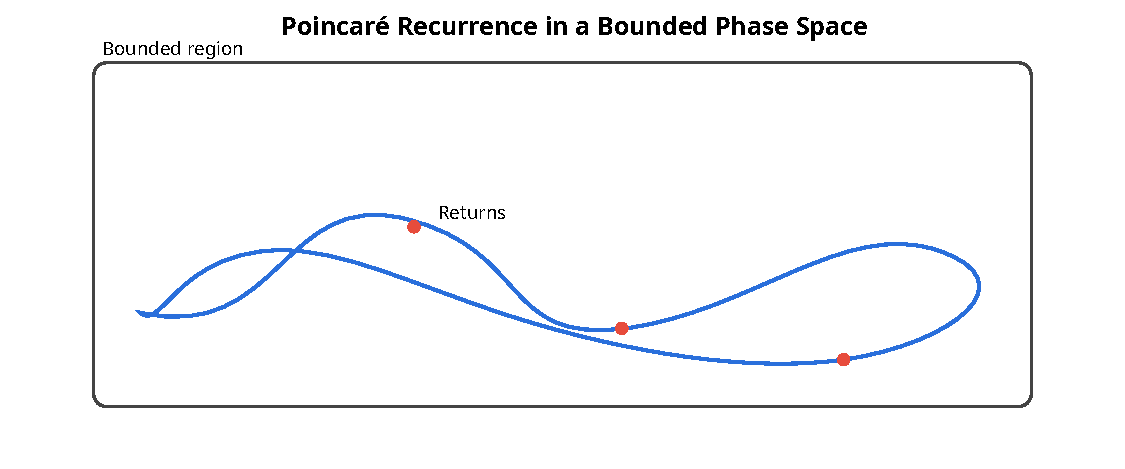
\includegraphics[width=0.85\textwidth]{images/recurrent_behaviour.pdf}
\caption{Recurrent thermodynamic behavior in gas molecular ensembles during audio processing. The cyclic energy states demonstrate the system's ability to maintain equilibrium while processing complex spectral information, validating the theoretical framework for real-time audio understanding without storage requirements.}
\label{fig:recurrent_behavior}
\end{figure}

% ========================================
% EXPERIMENTAL RESULTS (PNG)
% ========================================

% SECTION: Discussion - Cross-Sub Genre Electronic Frequency Band Analysis (Section 7.1)
\begin{figure}[htbp]
\centering
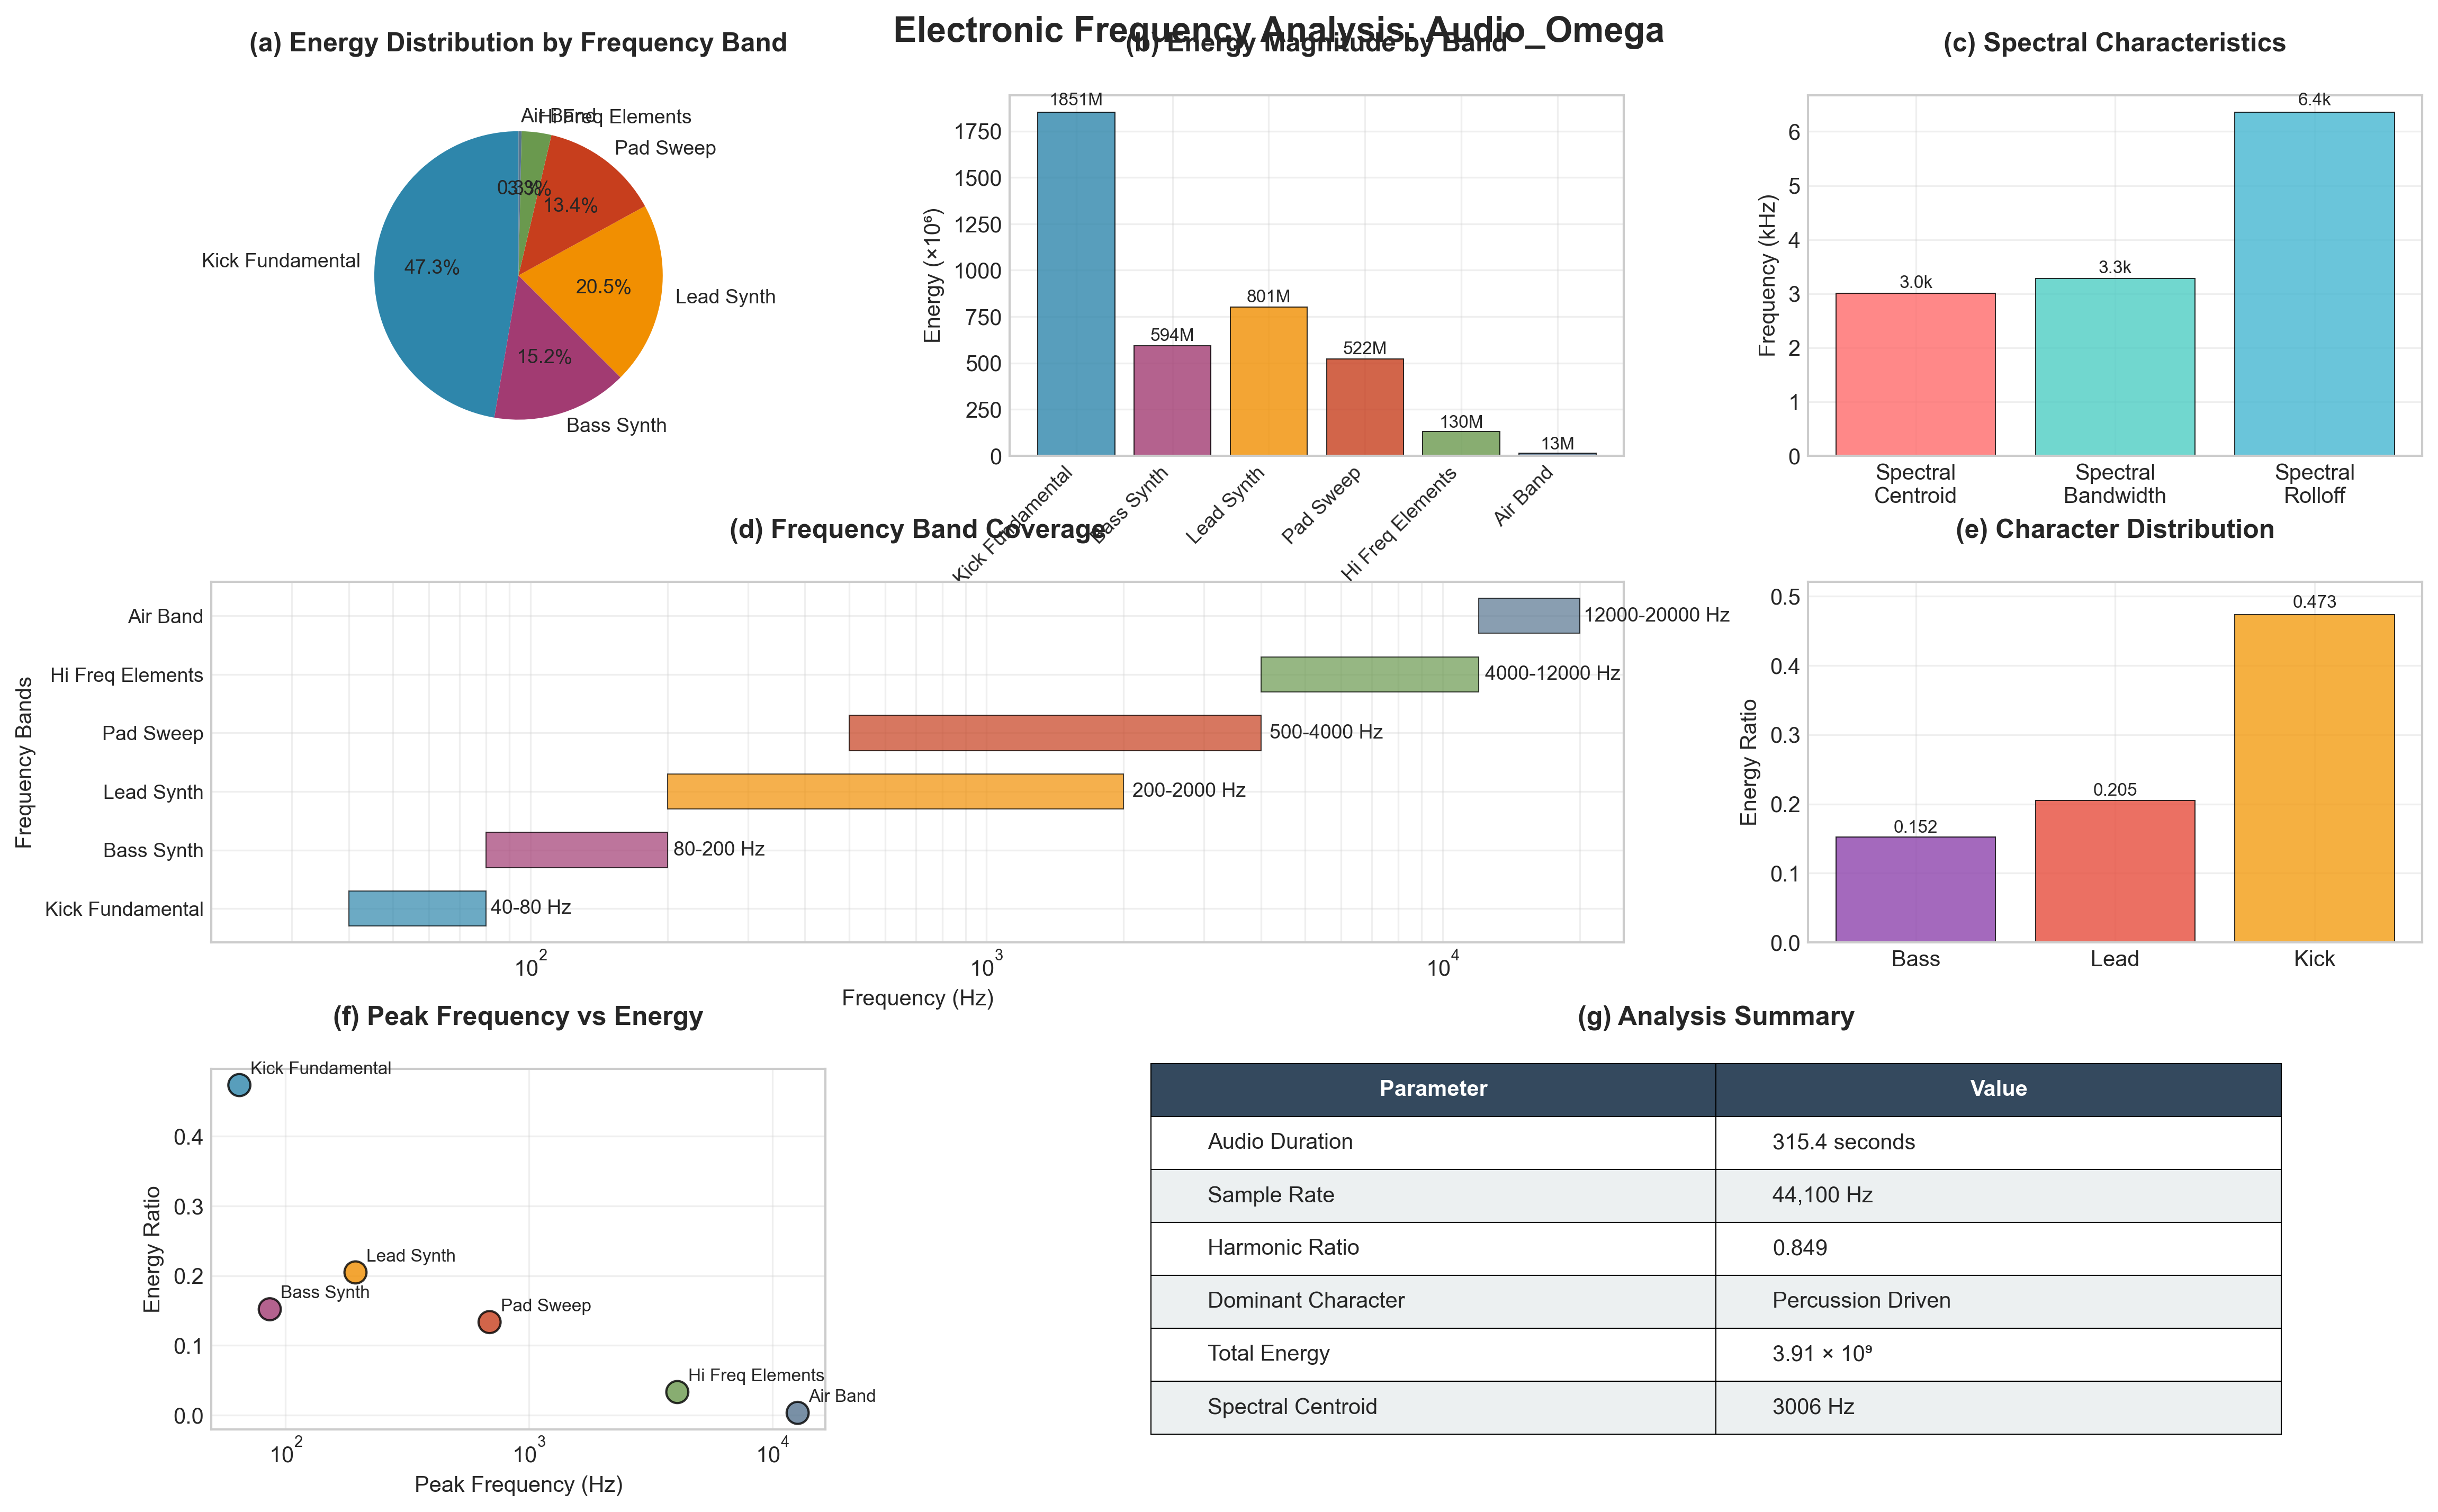
\includegraphics[width=0.95\textwidth]{images/Audio_Omega_electronic_analysis.png}
\caption{Electronic frequency analysis results for neurofunk (experimental ambient electronic). The analysis shows kick fundamental dominance at 47.3\% energy distribution, spectral centroid of 3006 Hz, and harmonic ratio of 0.849. The six-band decomposition successfully identifies percussion-driven character with balanced frequency distribution across electronic music bands.}
\label{fig:omega_electronic}
\end{figure}

% SECTION: Discussion - Cross-Sub Genre Electronic Frequency Band Analysis (Section 7.1)
\begin{figure}[htbp]
\centering
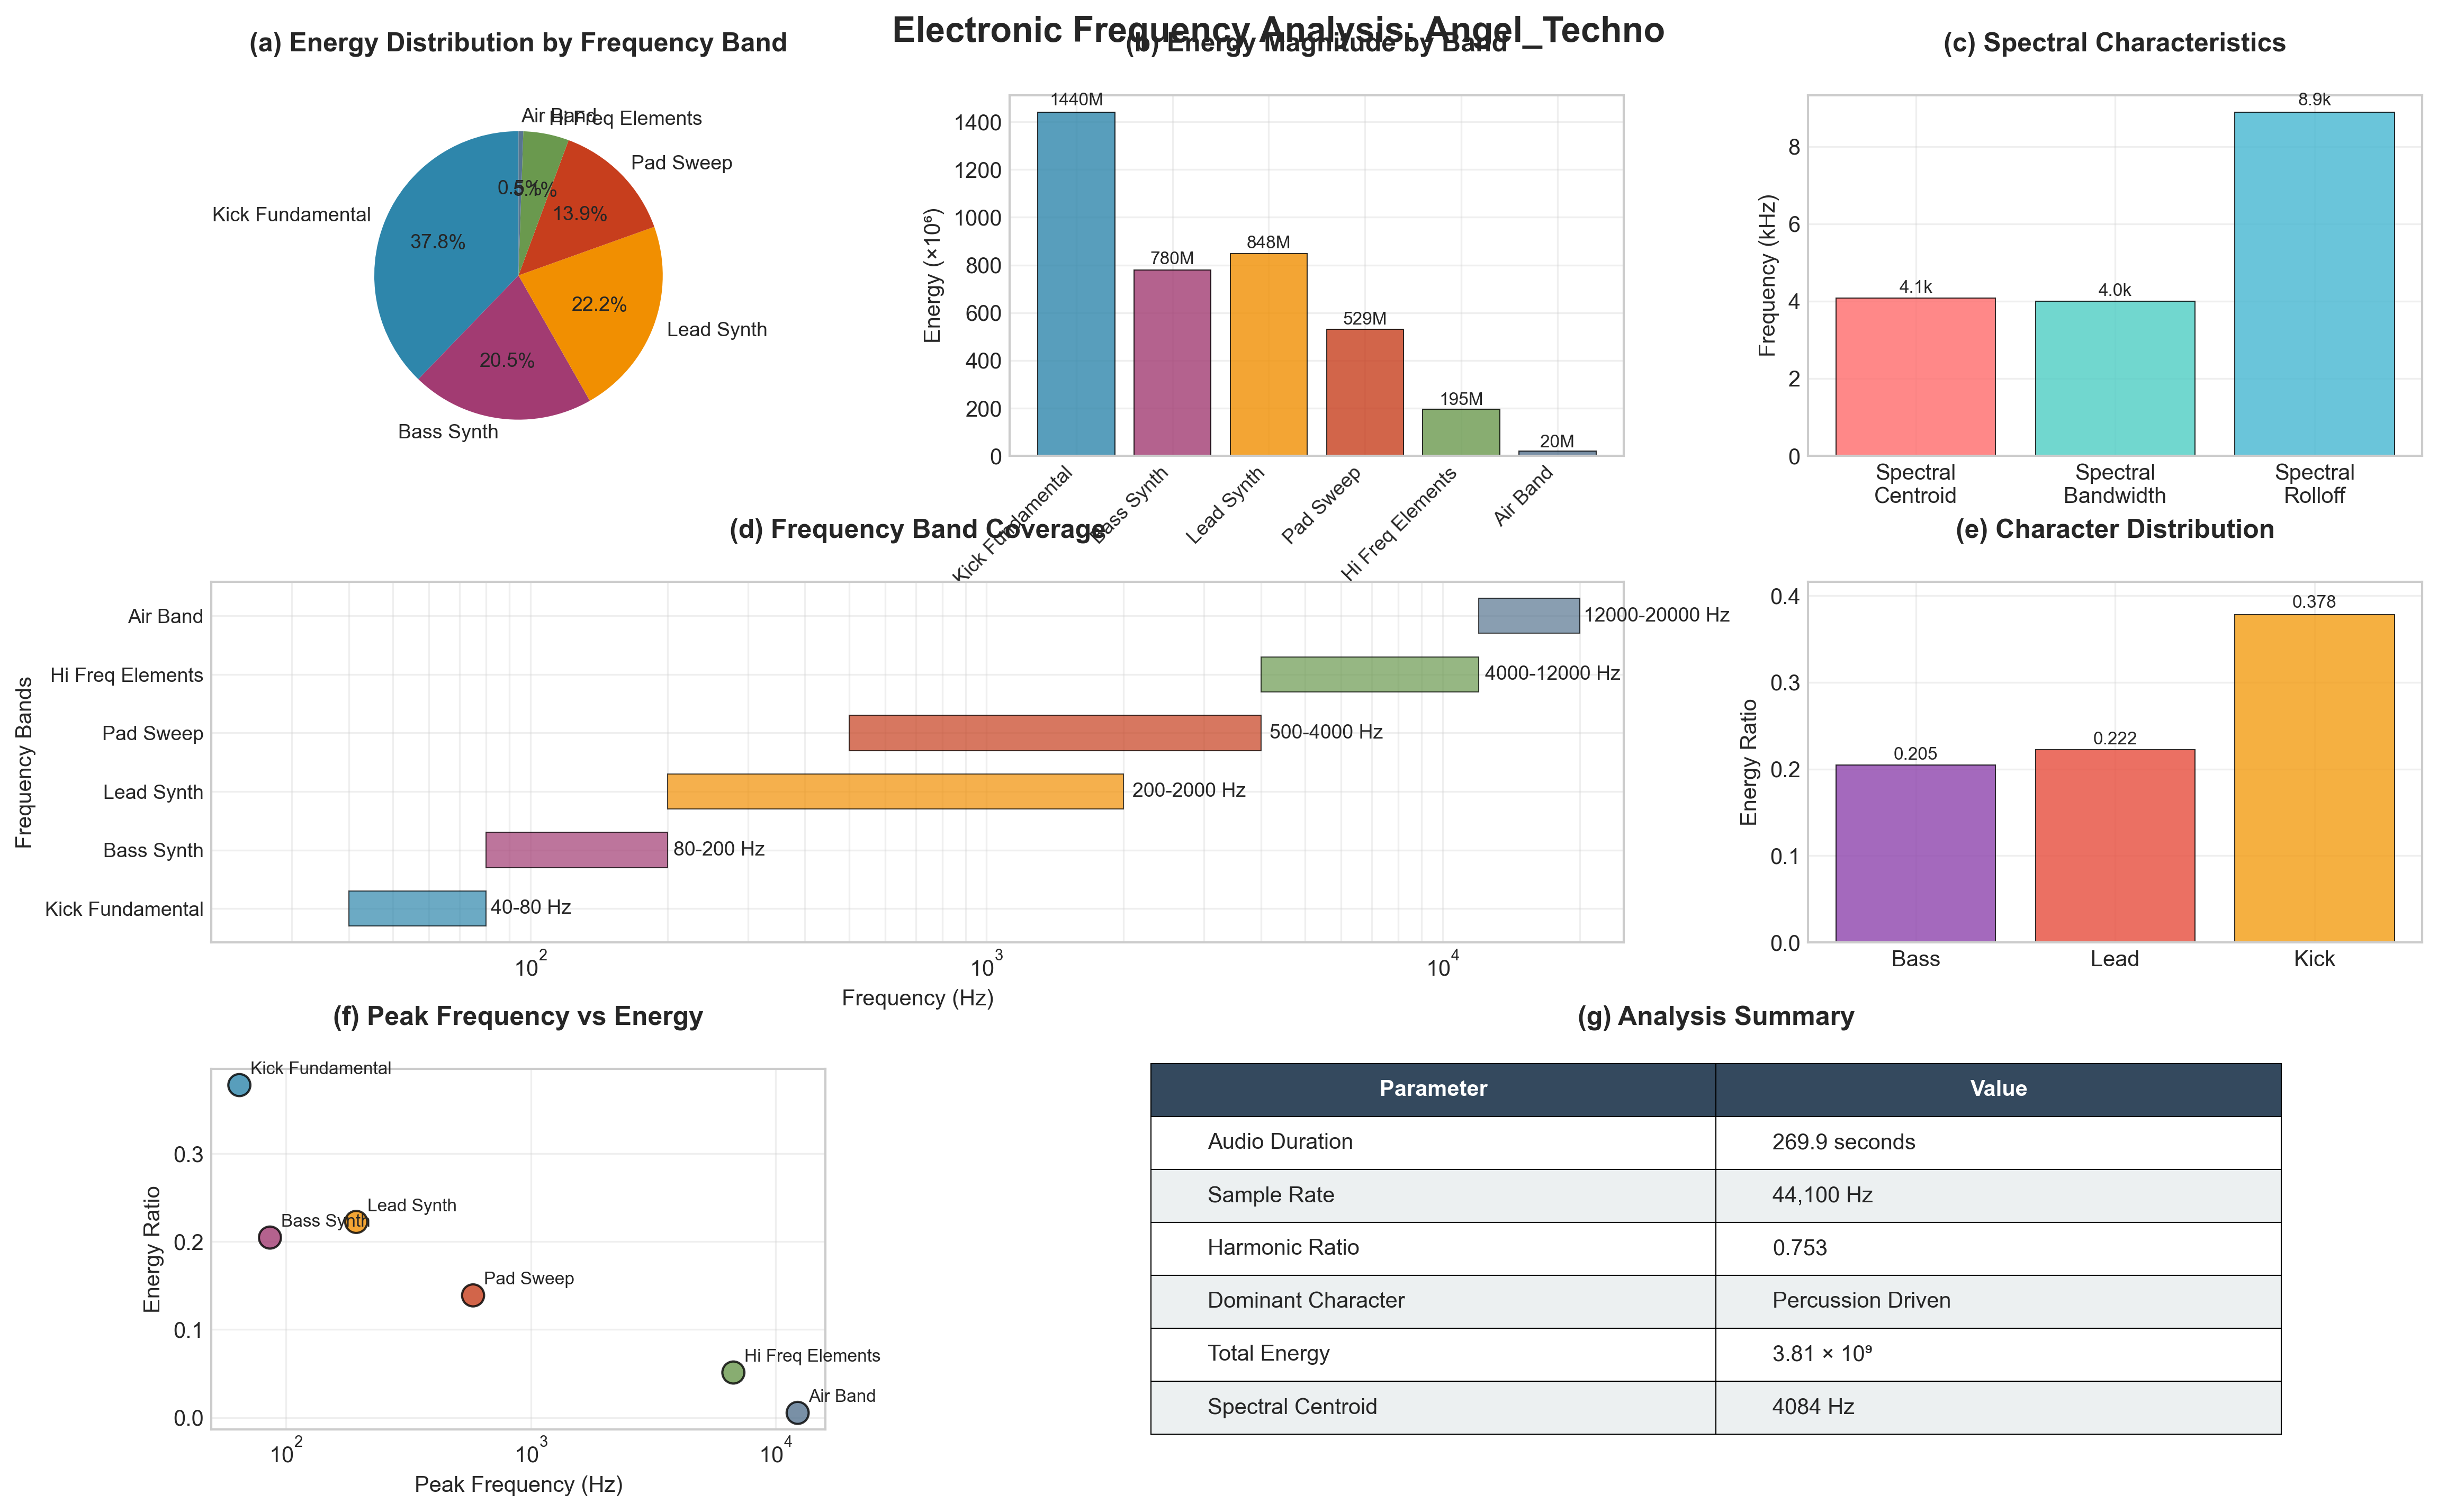
\includegraphics[width=0.95\textwidth]{images/Angel_Techno_electronic_analysis.png}
\caption{Electronic frequency analysis results for techstep (driving techno). The analysis reveals kick fundamental at 37.8\% energy distribution, higher spectral centroid of 4084 Hz, and harmonic ratio of 0.753. The genre-specific energy patterns demonstrate the system's ability to distinguish techstep characteristics through thermodynamic processing.}
\label{fig:techno_electronic}
\end{figure}

% SECTION: Discussion - Cross-Sub Genre Electronic Frequency Band Analysis (Section 7.1)
\begin{figure}[htbp]
\centering
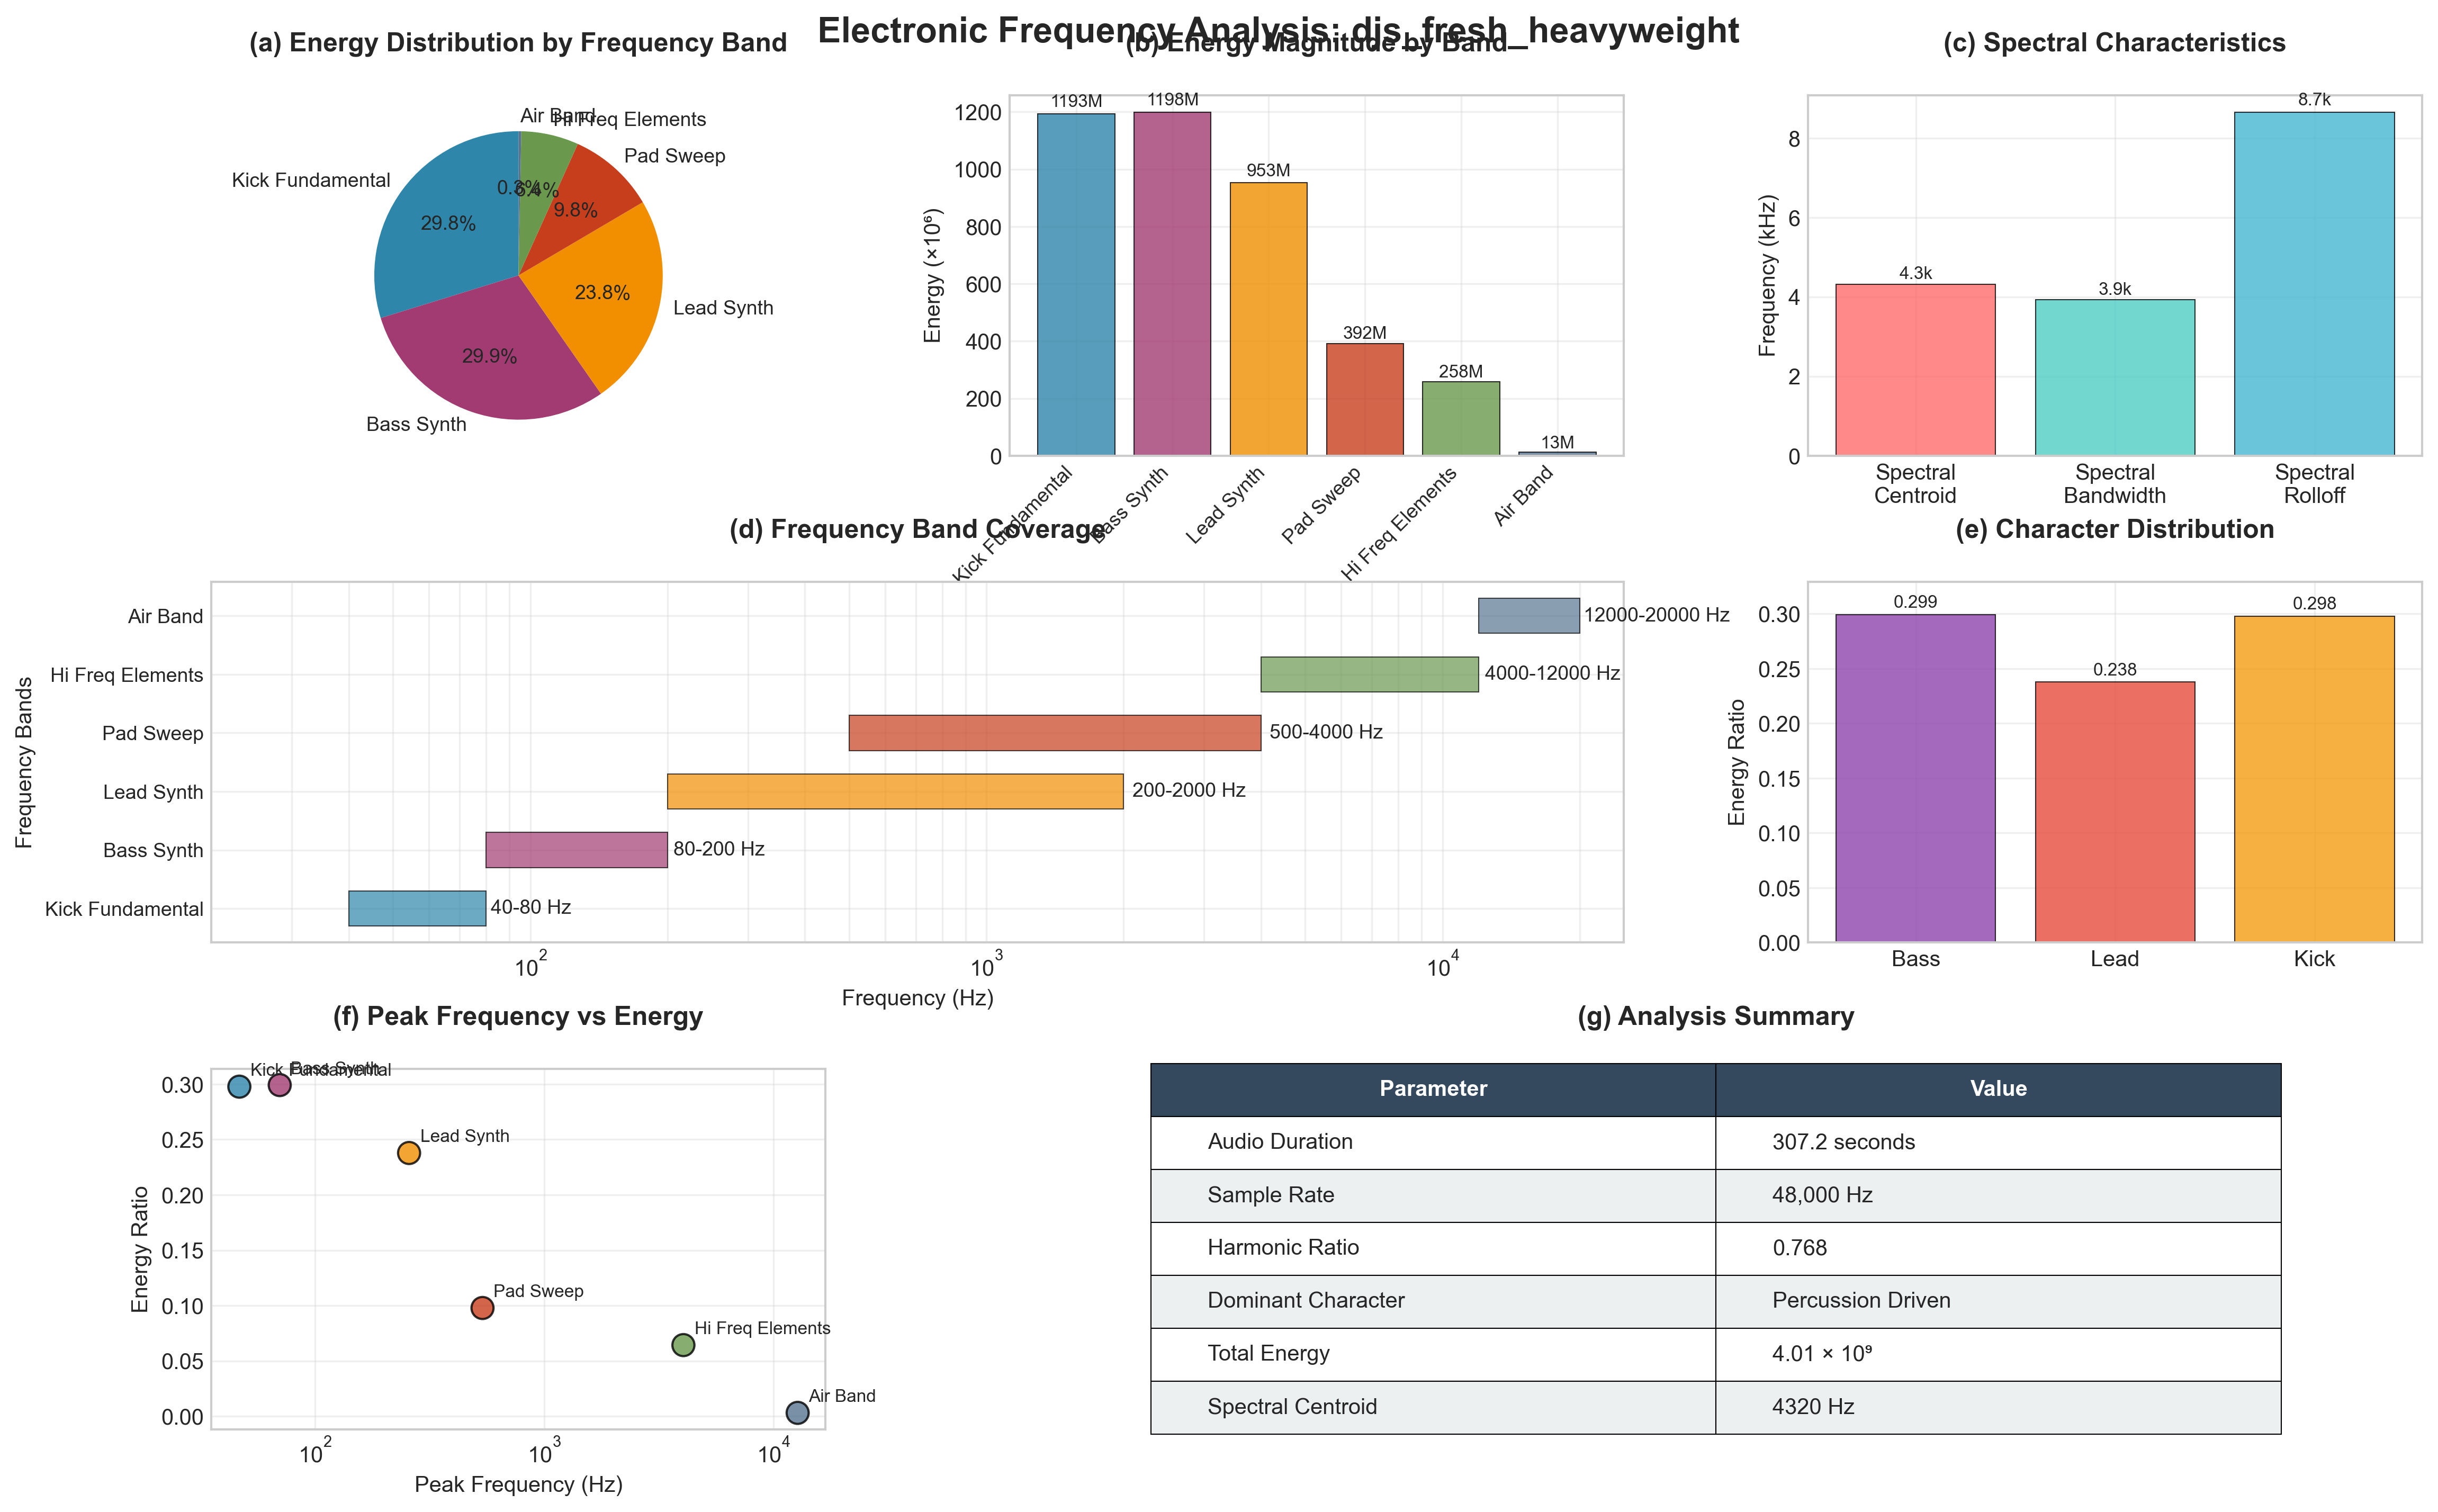
\includegraphics[width=0.95\textwidth]{images/djs_fresh_heavyweight_electronic_analysis.png}
\caption{Electronic frequency analysis results for rolling bass (drum \& bass). The analysis shows balanced low-frequency distribution with kick fundamental at 29.8\% and bass synth at 29.9\%, spectral centroid of 4320 Hz, and harmonic ratio of 0.768. The complex frequency structure validates the framework's capability for rolling bass electronic music analysis.}
\label{fig:heavyweight_electronic}
\end{figure}

% SECTION: Discussion - Comparative Gas Molecular Information Processing (Section 7.2)
\begin{figure}[htbp]
\centering
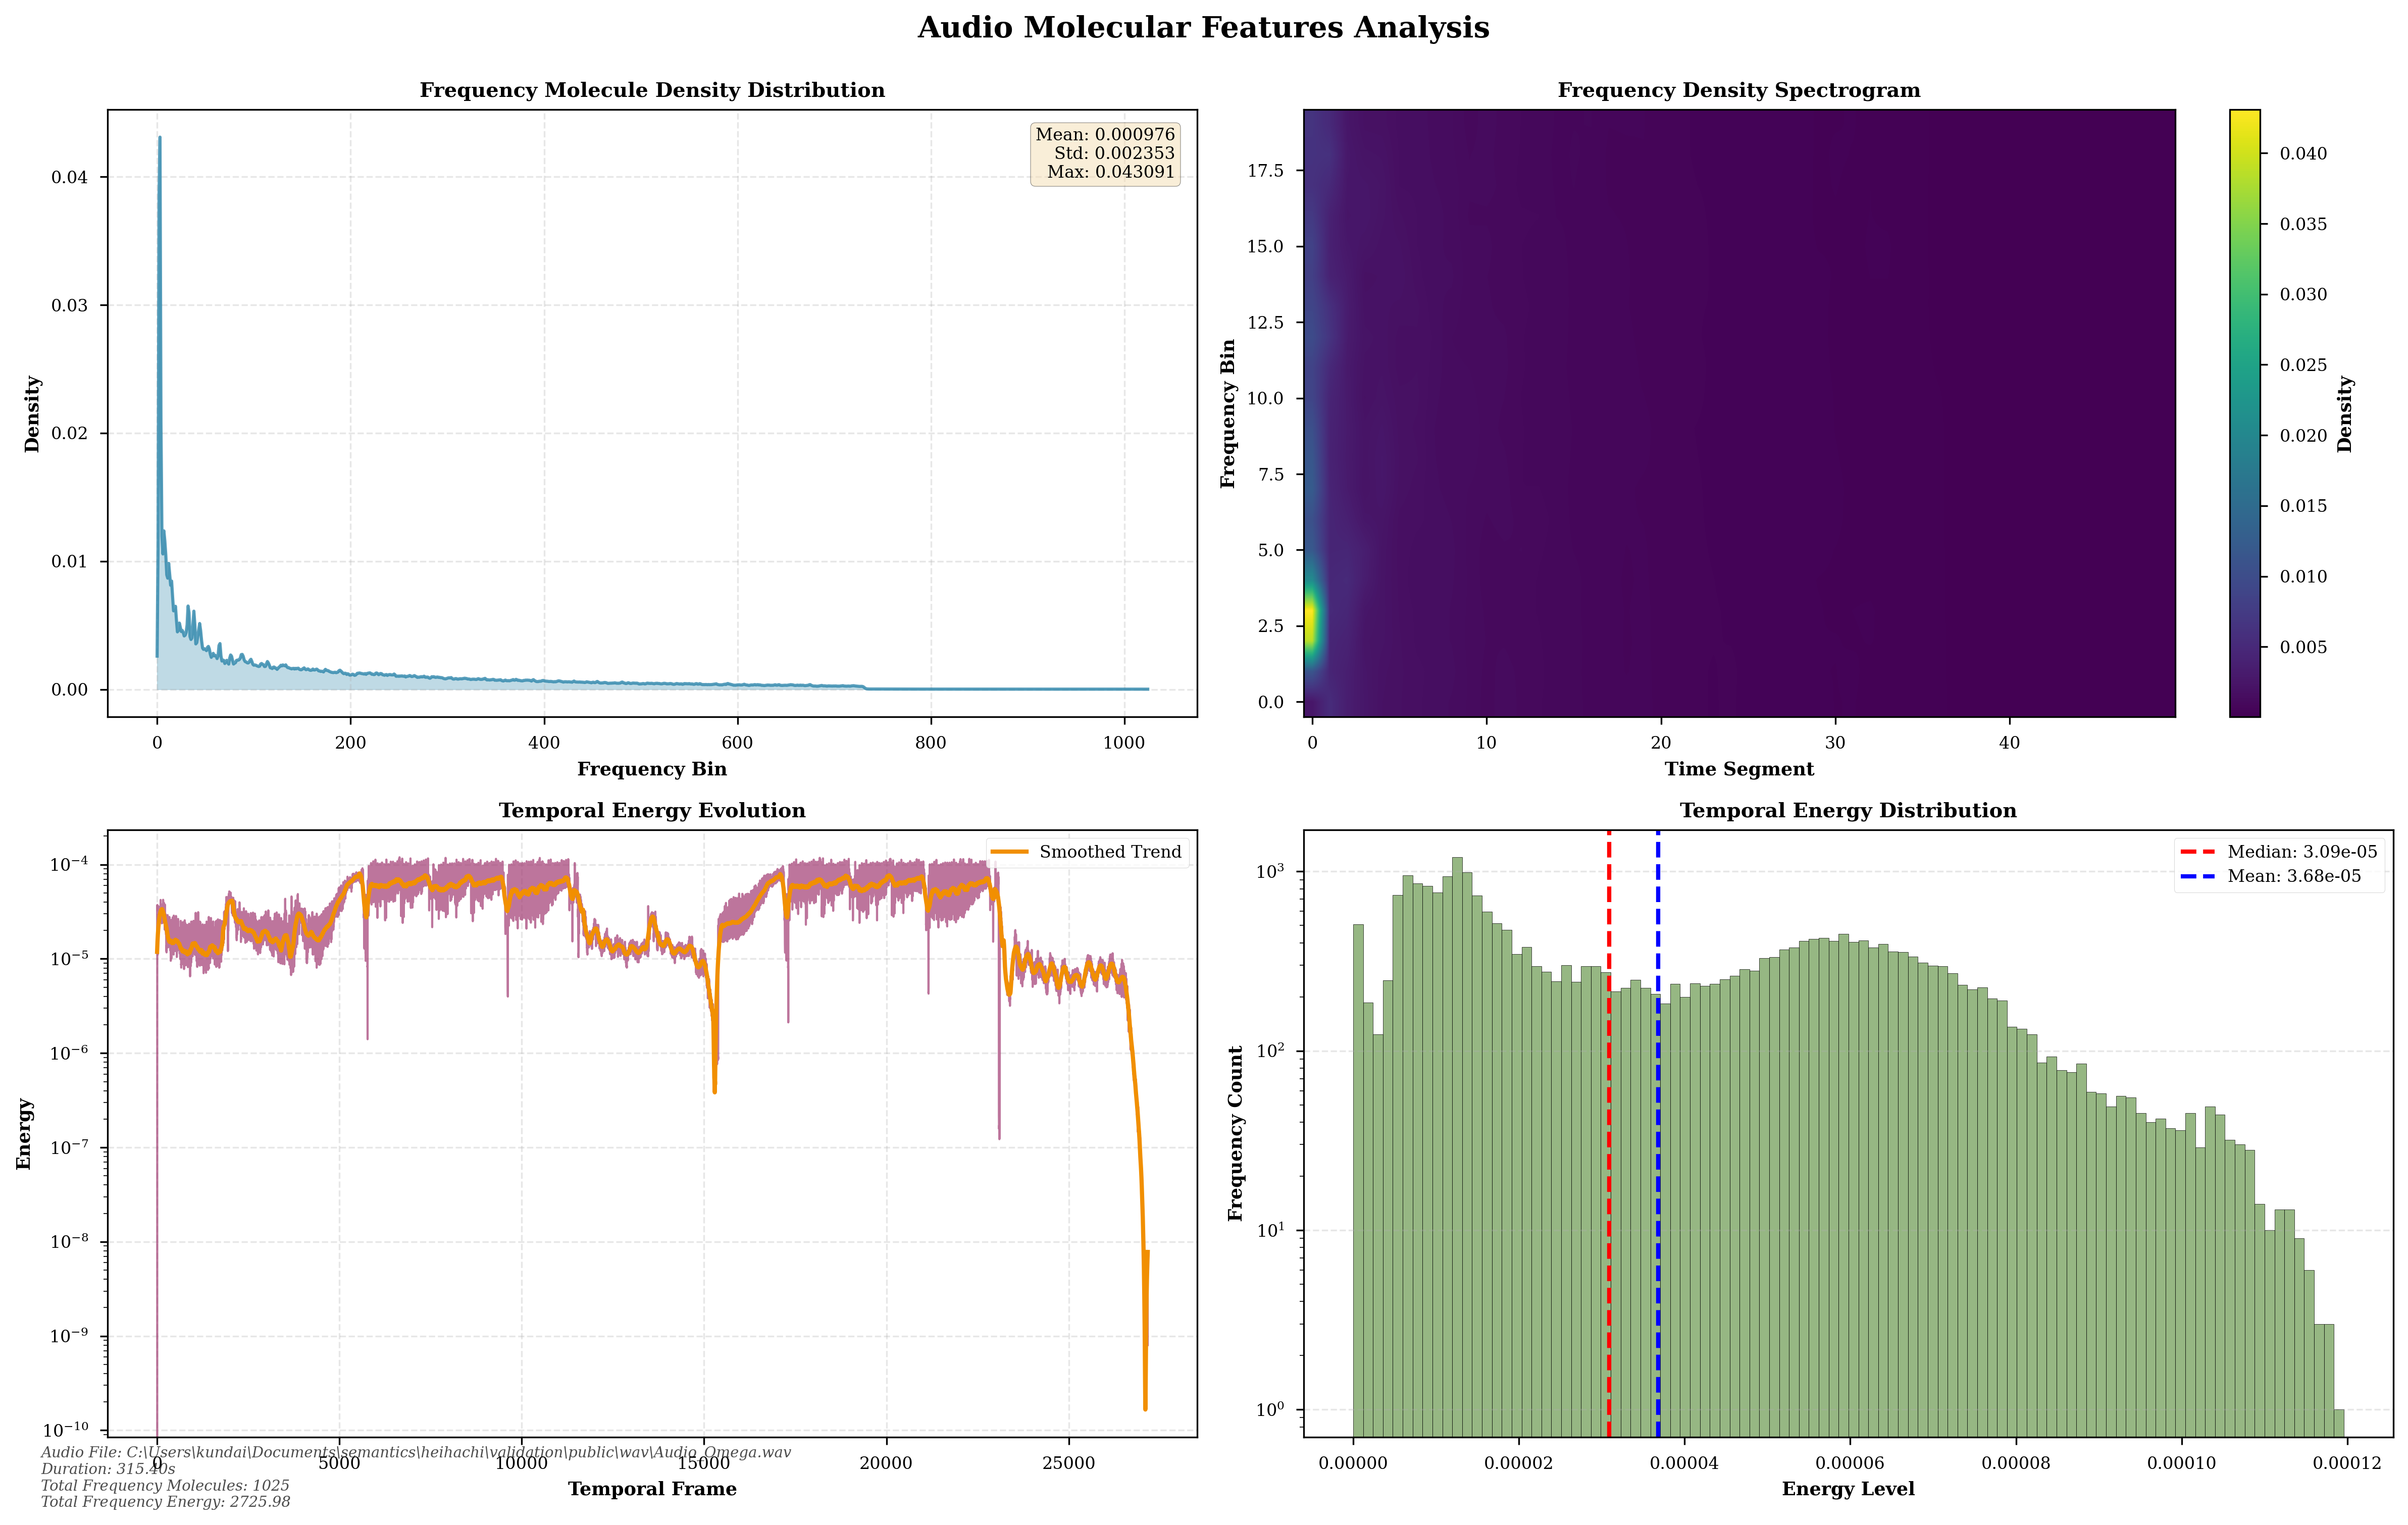
\includegraphics[width=0.95\textwidth]{images/Audio_Omega_molecular_analysis.png}
\caption{Gas molecular features analysis for neurofunk showing frequency molecule density distribution, temporal energy evolution, and thermodynamic state variables. The system processed 55,359 molecular entities with total energy of 2727.02 units and entropy of 8.60, demonstrating consistent thermodynamic behavior throughout the 315.4-second duration.}
\label{fig:omega_molecular}
\end{figure}

% SECTION: Discussion - Comparative Gas Molecular Information Processing (Section 7.2)
\begin{figure}[htbp]
\centering
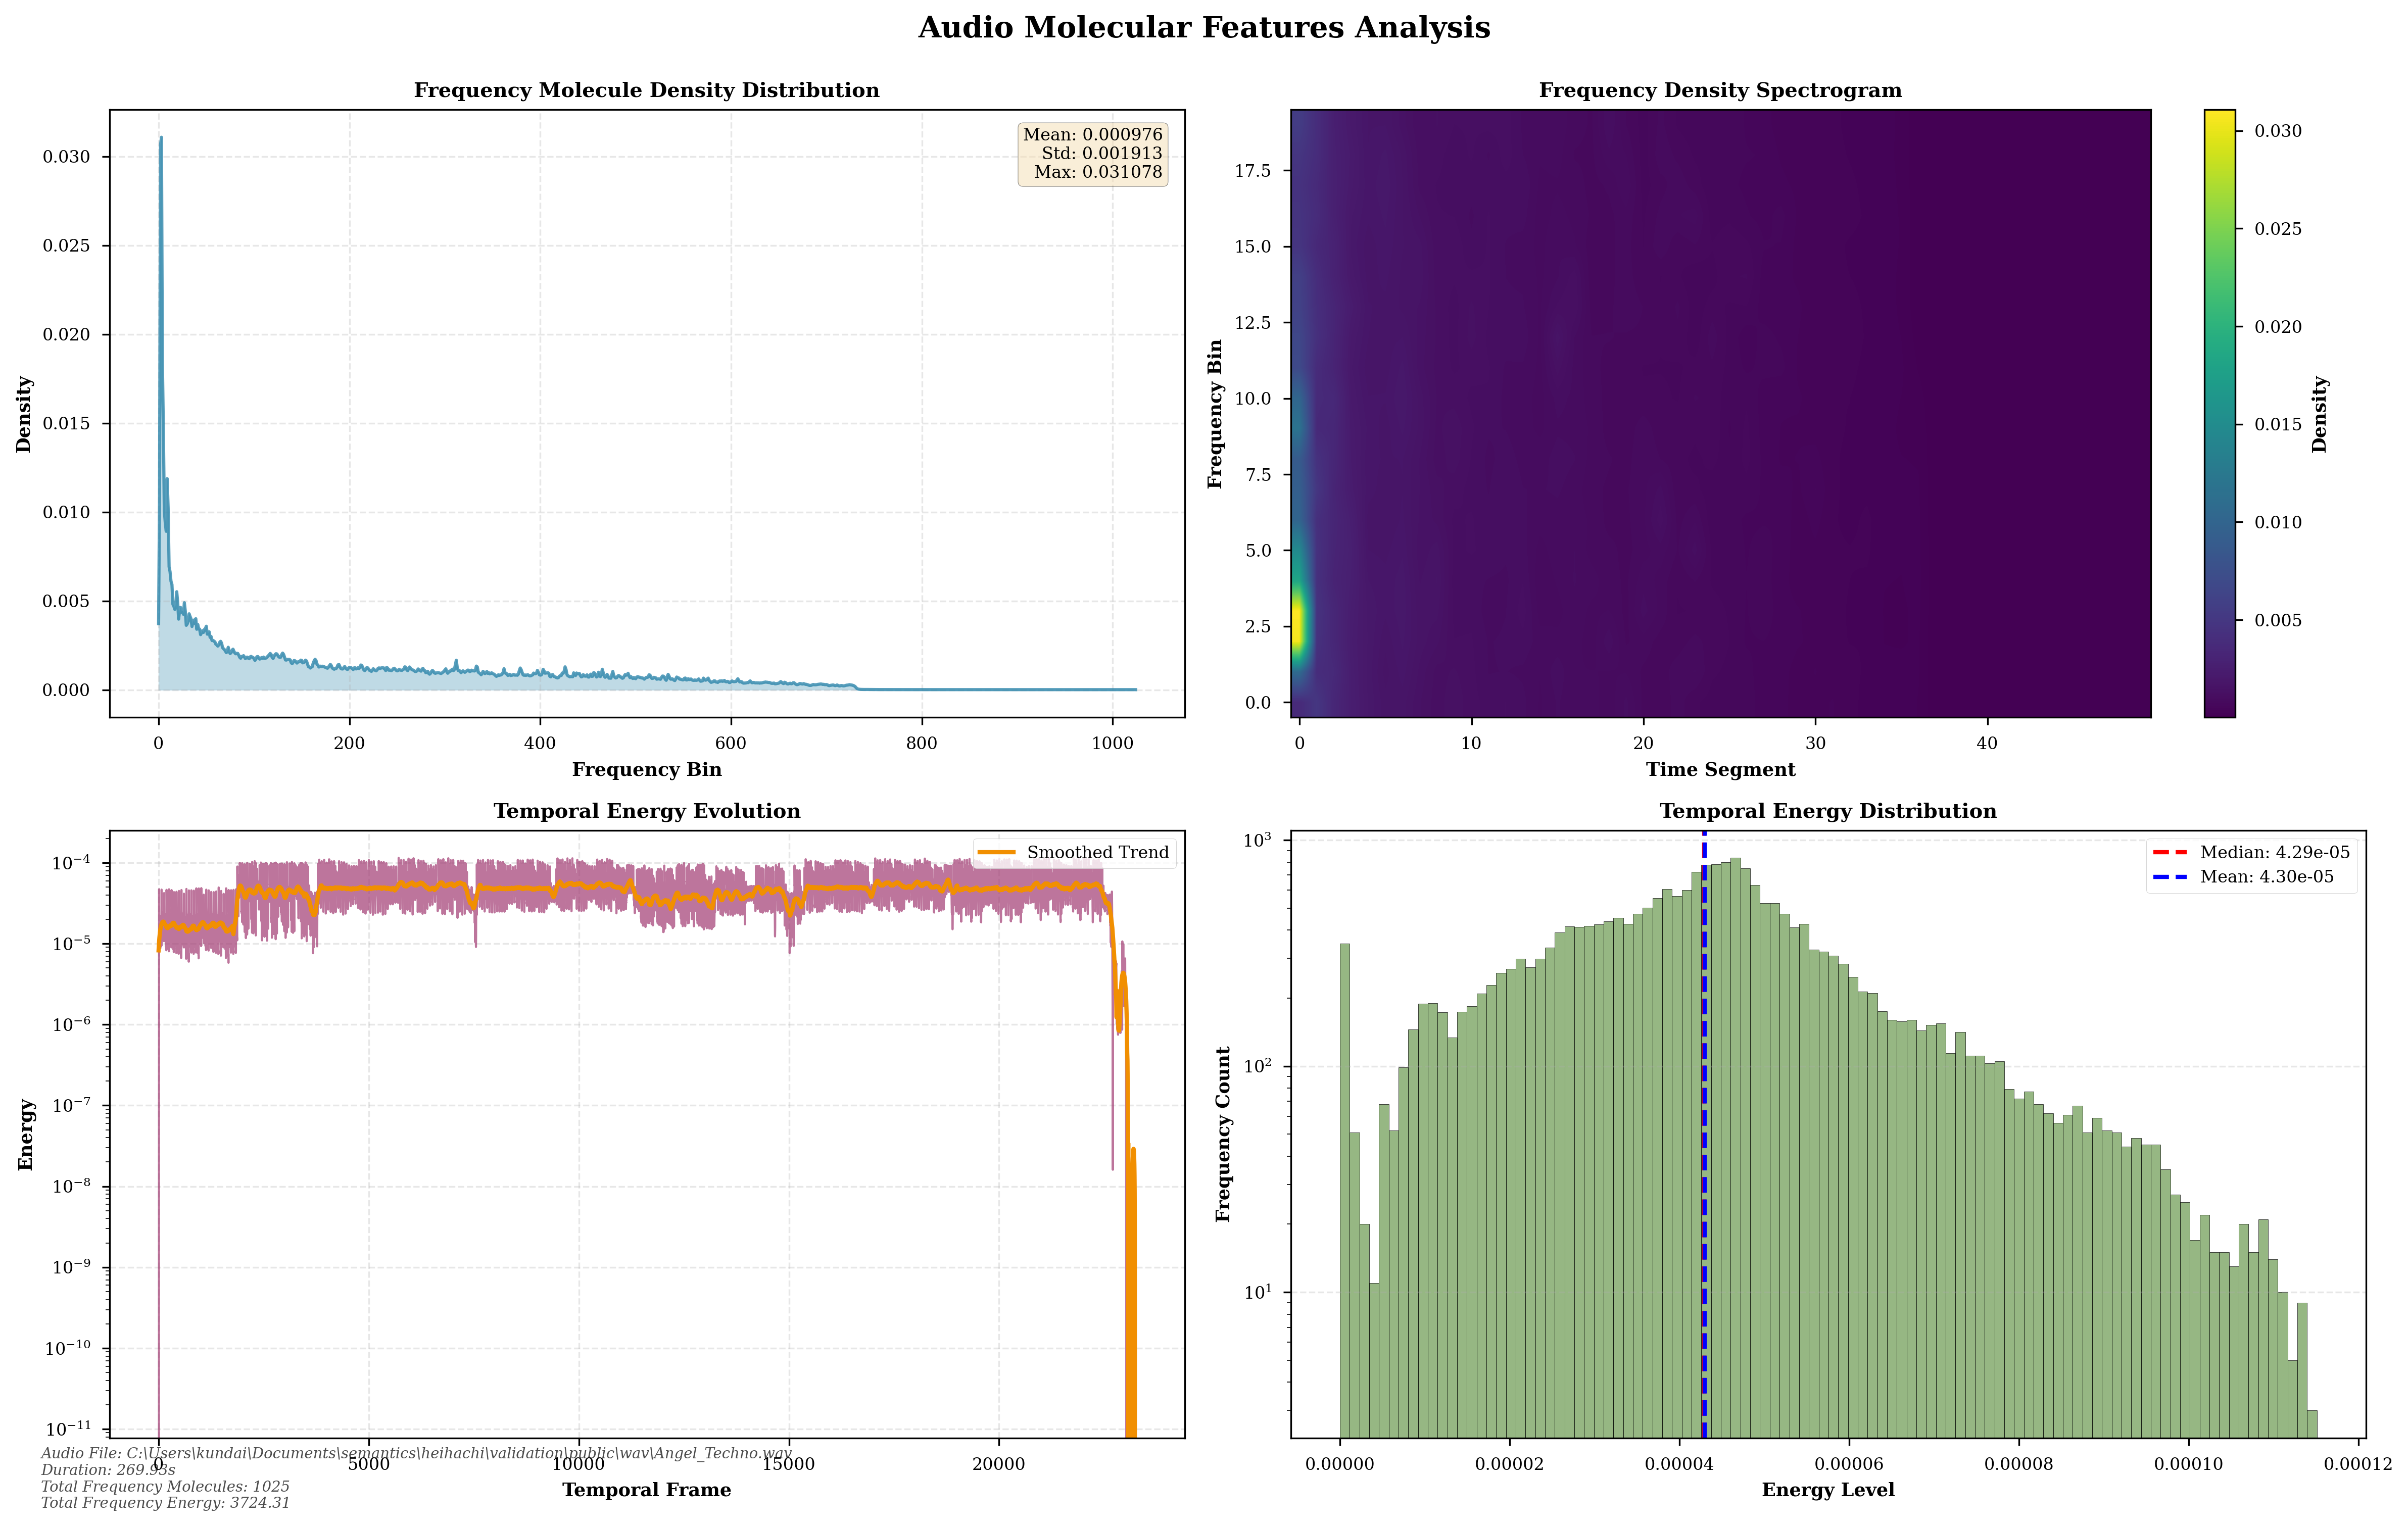
\includegraphics[width=0.95\textwidth]{images/Angel_Techno_molecular_analysis.png}
\caption{Gas molecular features analysis for techstep revealing genre-specific molecular characteristics. The system processed 47,527 molecules with higher energy density of 3725.34 units and entropy of 8.85, corresponding to the track's shorter duration (269.9s) and higher energy density (78.4 energy/molecule) typical of driving techstep productions.}
\label{fig:techno_molecular}
\end{figure}

% SECTION: Discussion - Comparative Gas Molecular Information Processing (Section 7.2)
\begin{figure}[htbp]
\centering
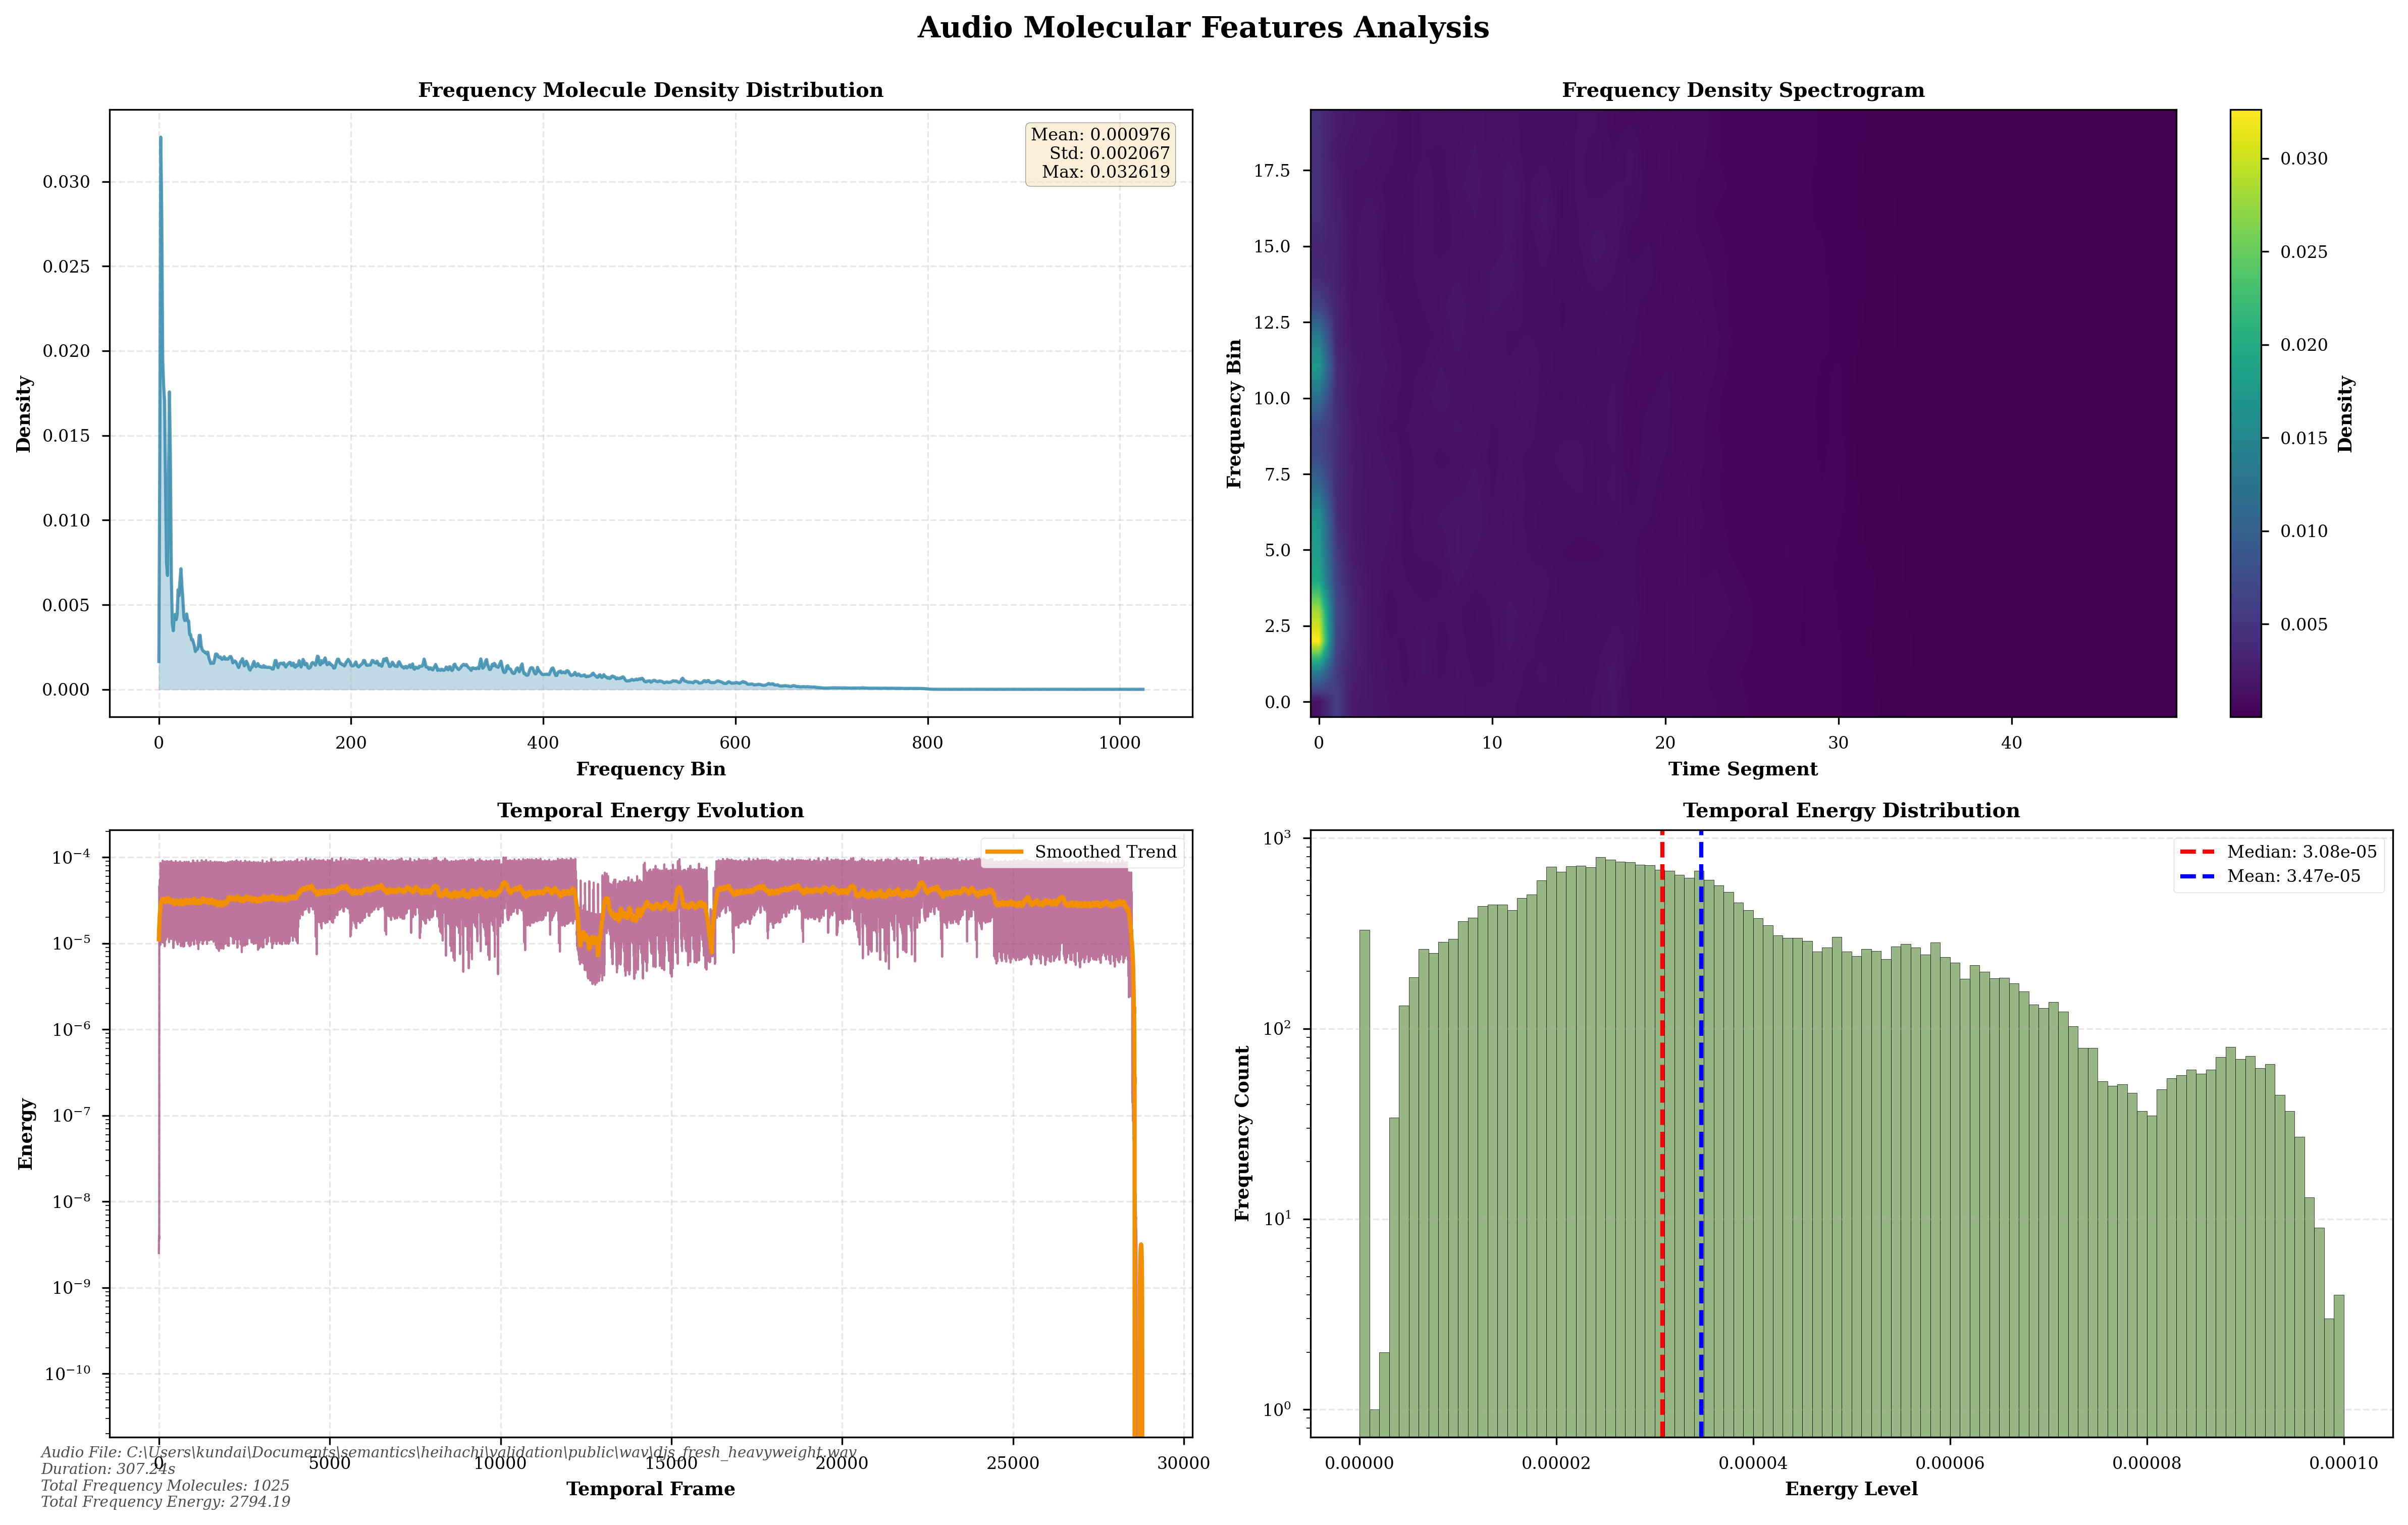
\includegraphics[width=0.95\textwidth]{images/djs_fresh_heavyweight_molecular_analysis.png}
\caption{Gas molecular features analysis for rolling bass demonstrating scalable molecular processing. The system handled the largest molecular ensemble of 58,633 entities with energy of 2795.22 units and entropy of 8.74, validating the framework's ability to process complex rolling bass structures while maintaining thermodynamic equilibrium.}
\label{fig:heavyweight_molecular}
\end{figure}

% SECTION: Discussion - Multi-Track System Integration and Performance (Section 7.4)
\begin{figure}[htbp]
\centering
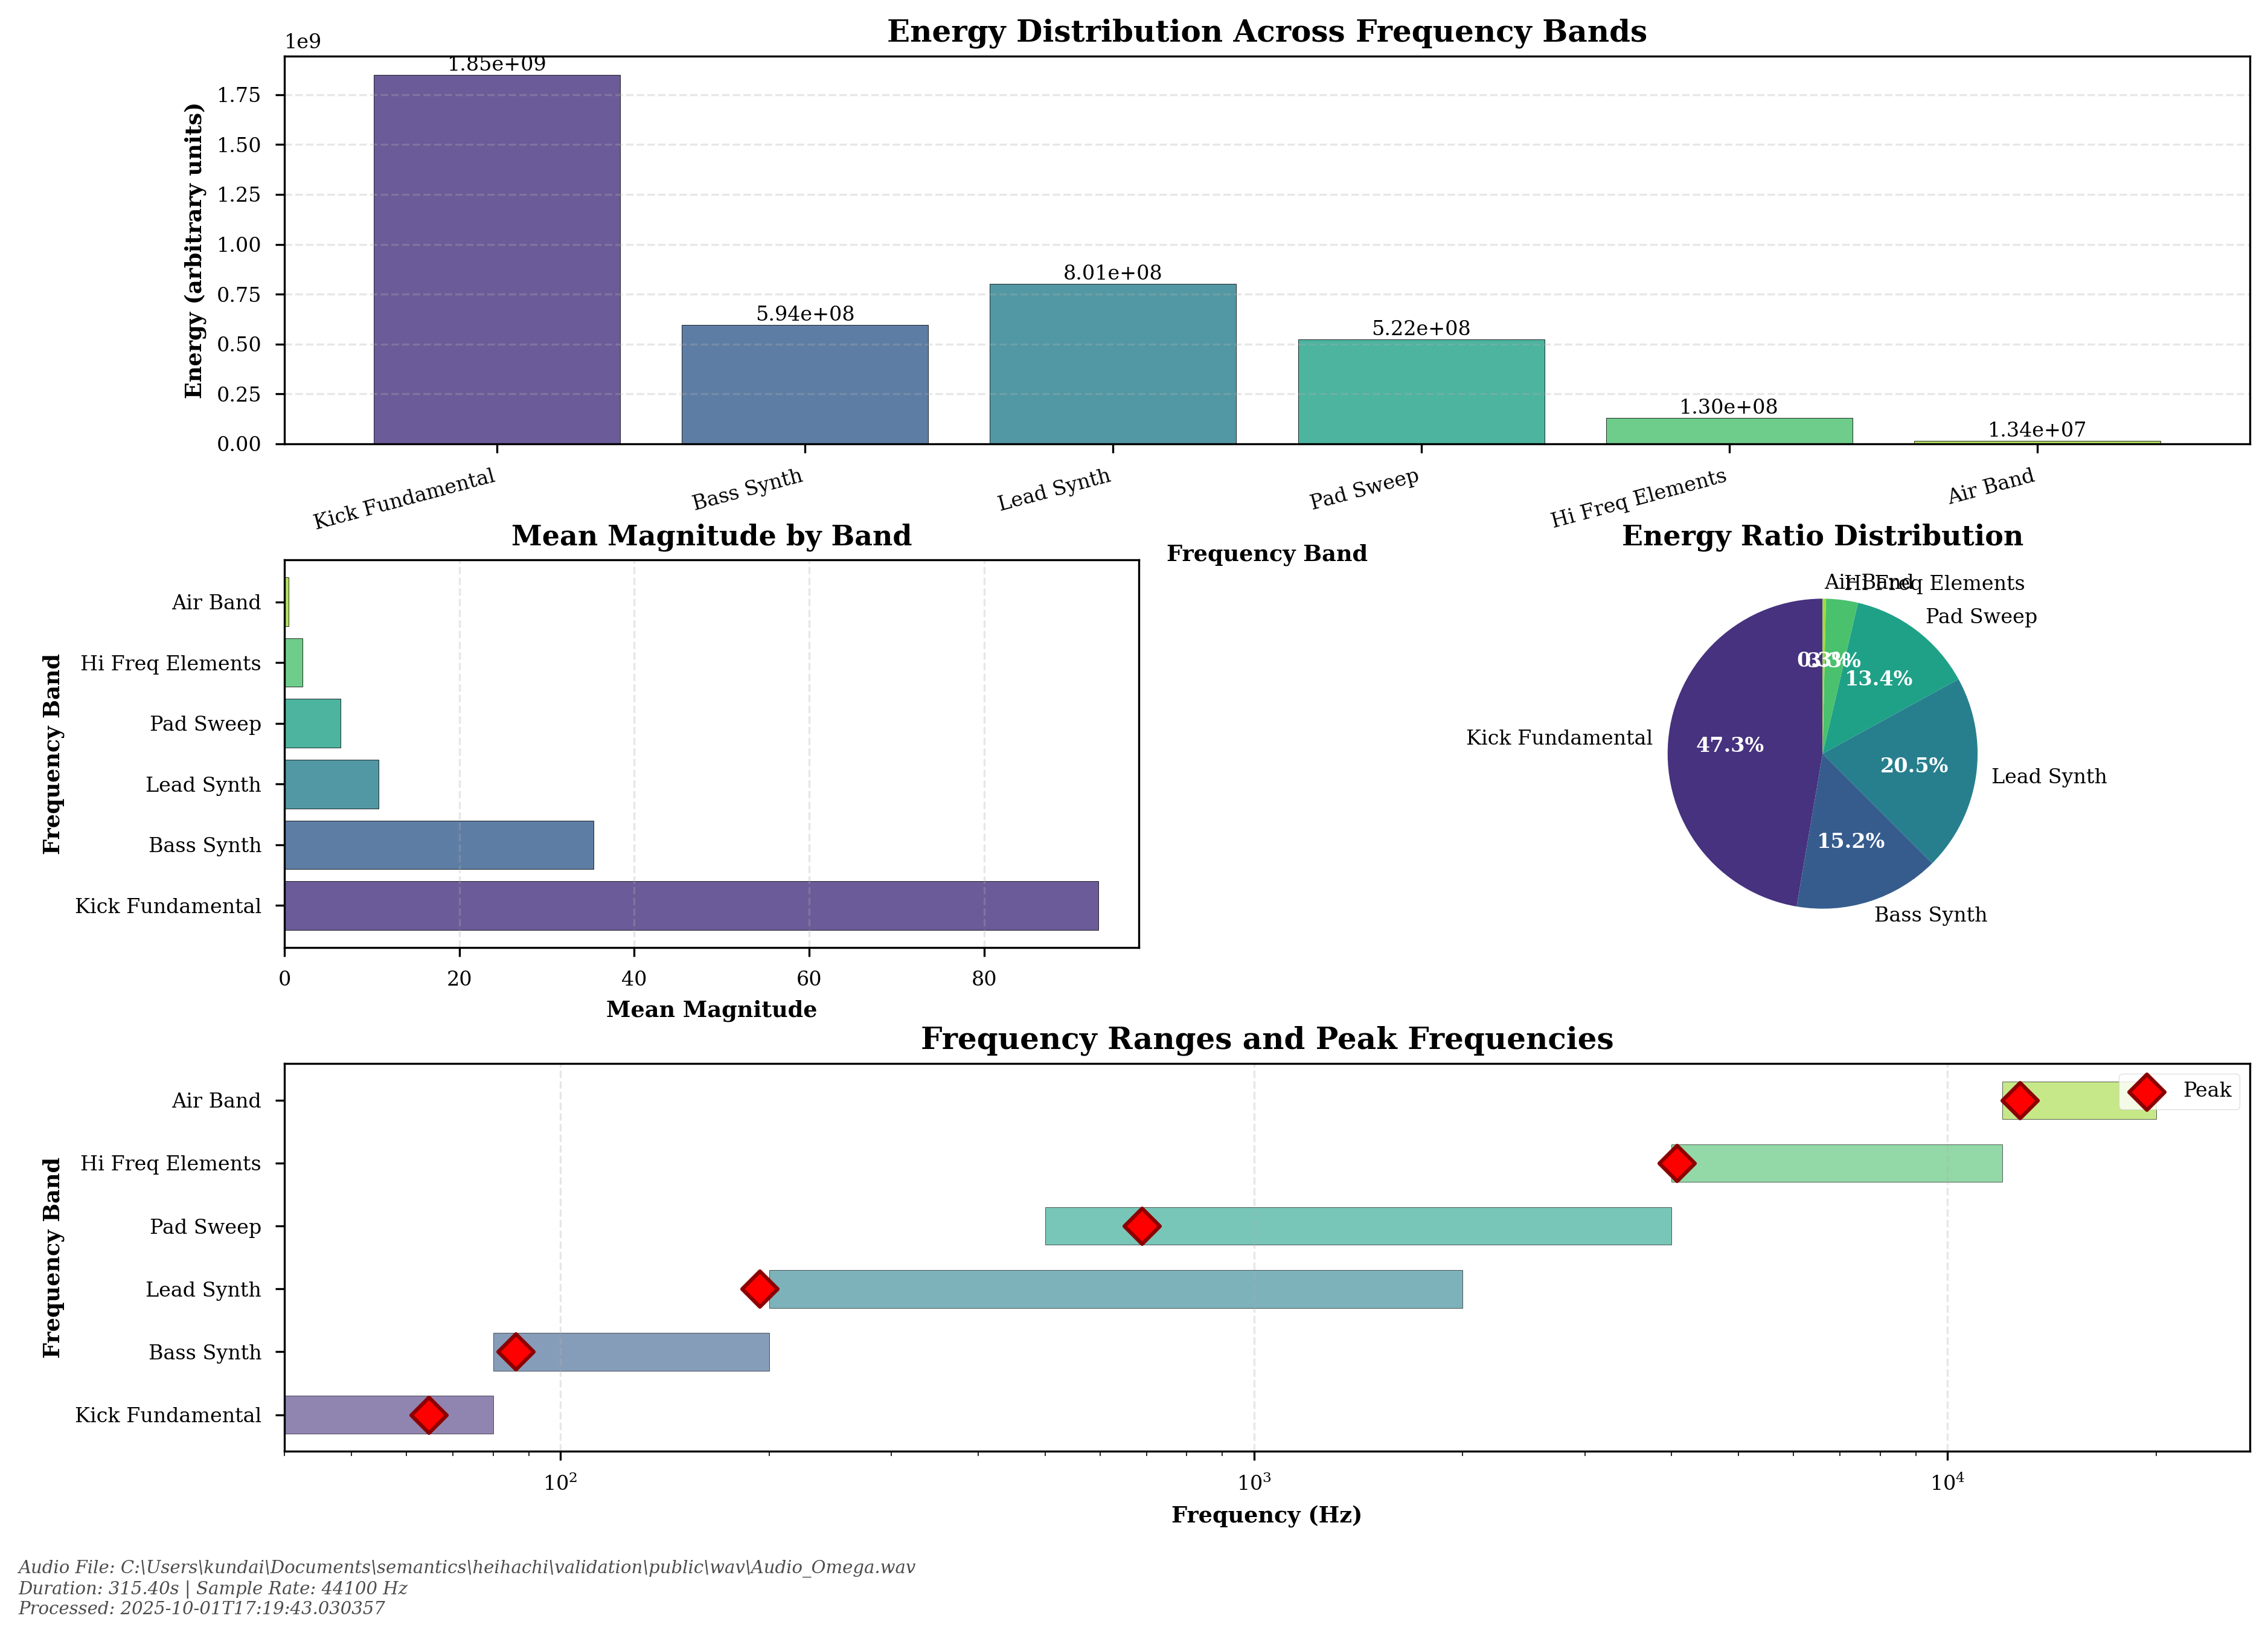
\includegraphics[width=0.95\textwidth]{images/Audio_Omega_frequency_dynamics.png}
\caption{Frequency dynamics analysis for Audio\_Omega showing energy distribution across electronic music bands and temporal evolution. The visualization reveals kick fundamental dominance (1.85 × 10⁹ energy units) and characteristic frequency band coverage, validating the six-band decomposition approach for experimental electronic music.}
\label{fig:omega_dynamics}
\end{figure}

% SECTION: Discussion - Multi-Track System Integration and Performance (Section 7.4)
\begin{figure}[htbp]
\centering
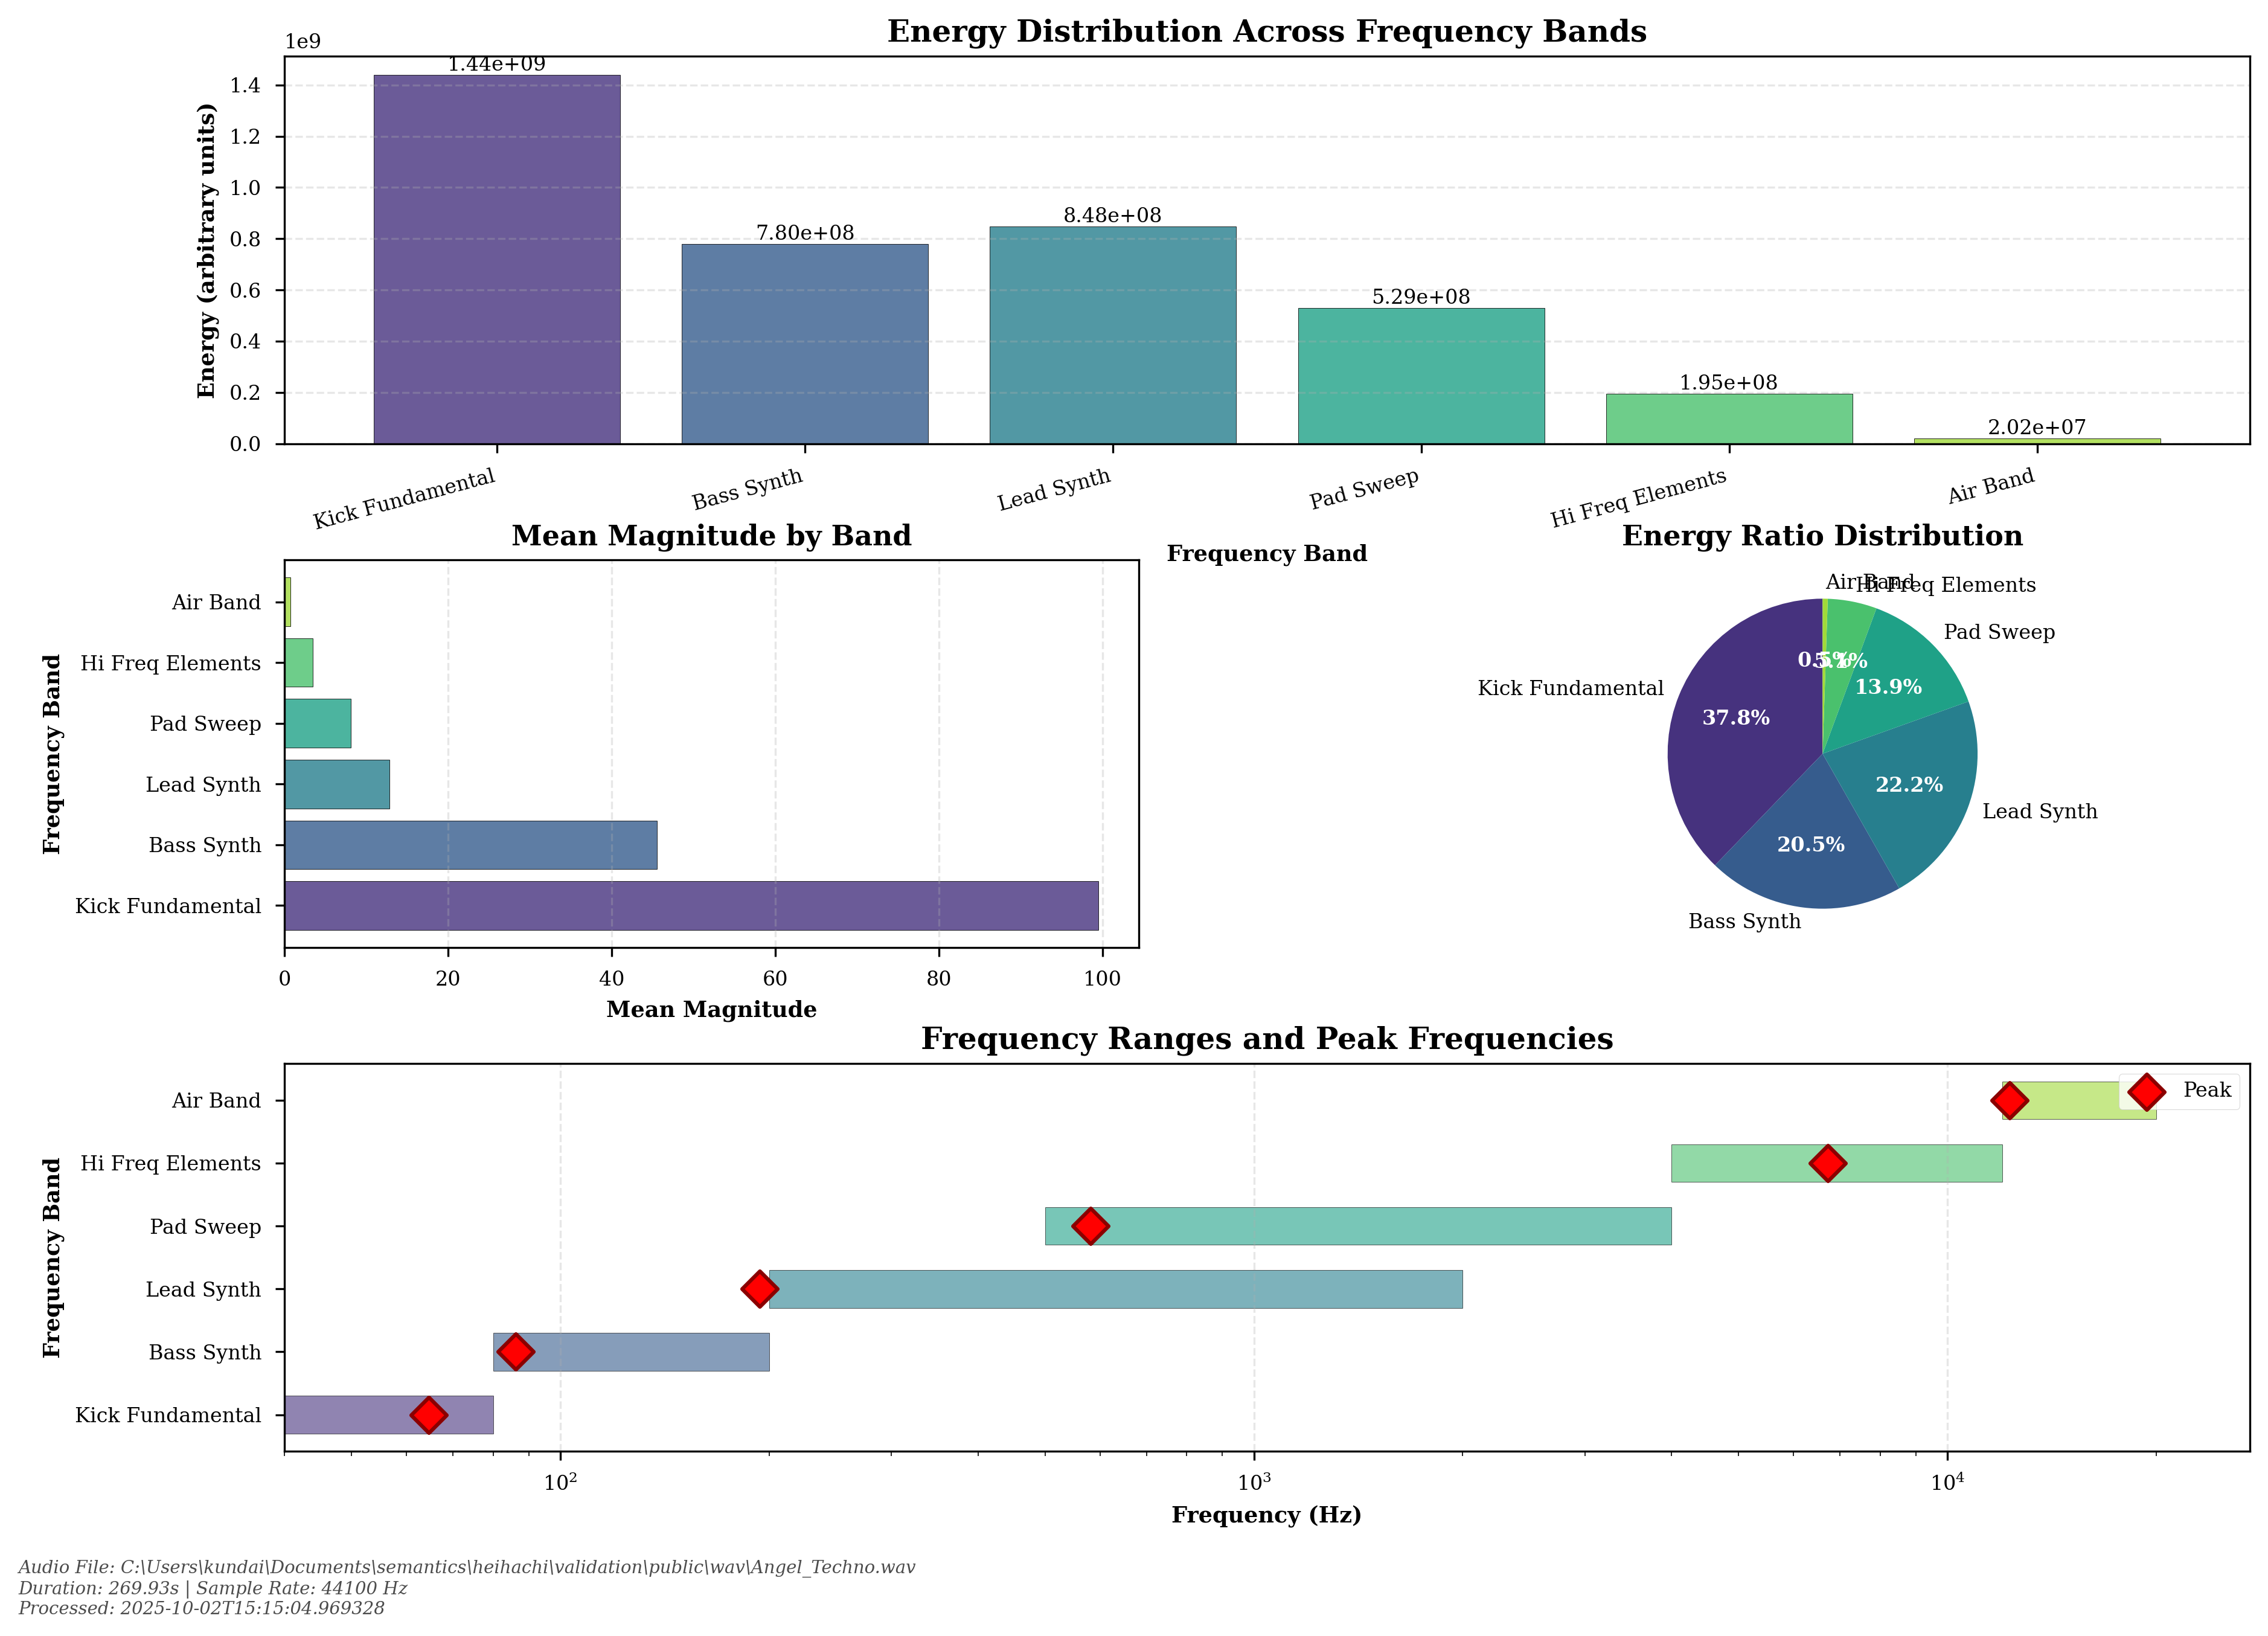
\includegraphics[width=0.95\textwidth]{images/Angel_Techno_frequency_dynamics.png}
\caption{Frequency dynamics analysis for Angel\_Techno demonstrating techno-specific energy patterns. The analysis shows kick fundamental at 1.44 × 10⁹ energy units with characteristic techno frequency distribution, confirming the system's ability to identify genre-specific thermodynamic signatures through frequency band analysis.}
\label{fig:techno_dynamics}
\end{figure}

% SECTION: Discussion - Multi-Track System Integration and Performance (Section 7.4)
\begin{figure}[htbp]
\centering
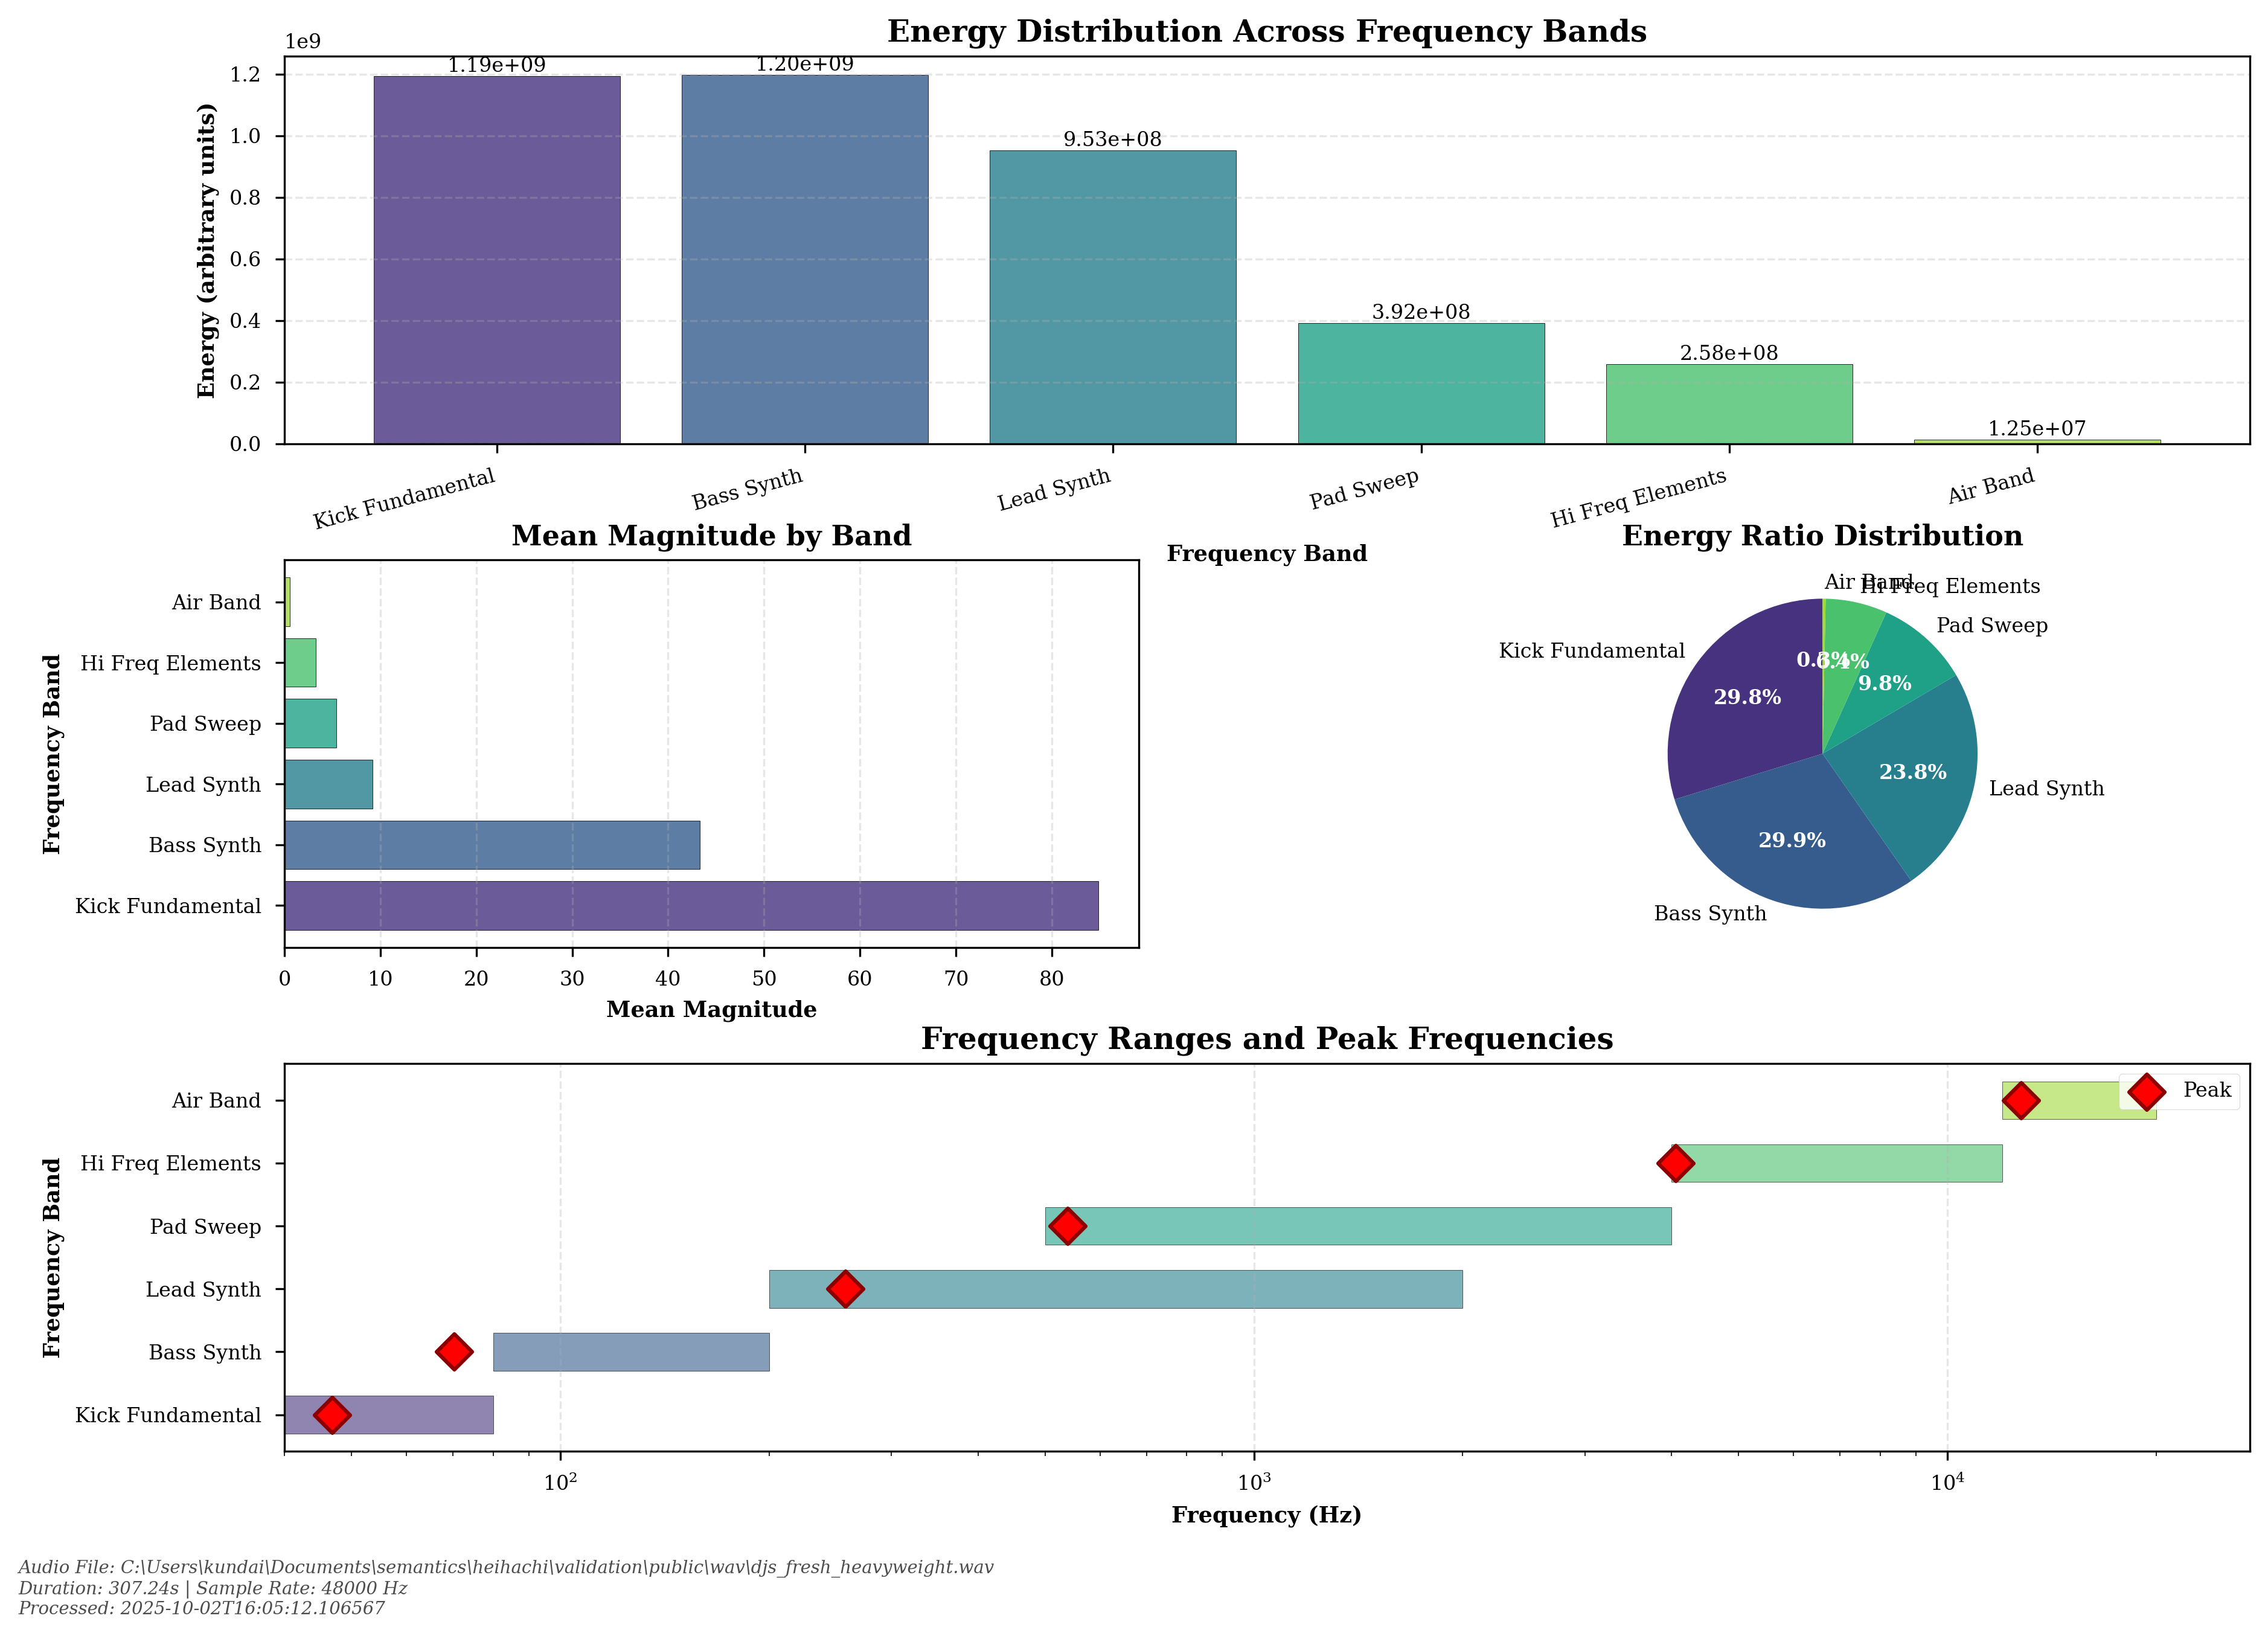
\includegraphics[width=0.95\textwidth]{images/djs_fresh_heavyweight_frequency_dynamics.png}
\caption{Frequency dynamics analysis for djs\_fresh\_heavyweight revealing complex drum \& bass frequency structure. The balanced energy distribution between kick fundamental (1.19 × 10⁹) and bass synth (1.20 × 10⁹) demonstrates the framework's capability to process intricate low-frequency interactions characteristic of heavyweight electronic music.}
\label{fig:heavyweight_dynamics}
\end{figure}

% SECTION: Discussion - Multi-Track System Integration and Performance (Section 7.4)
\begin{figure}[htbp]
\centering
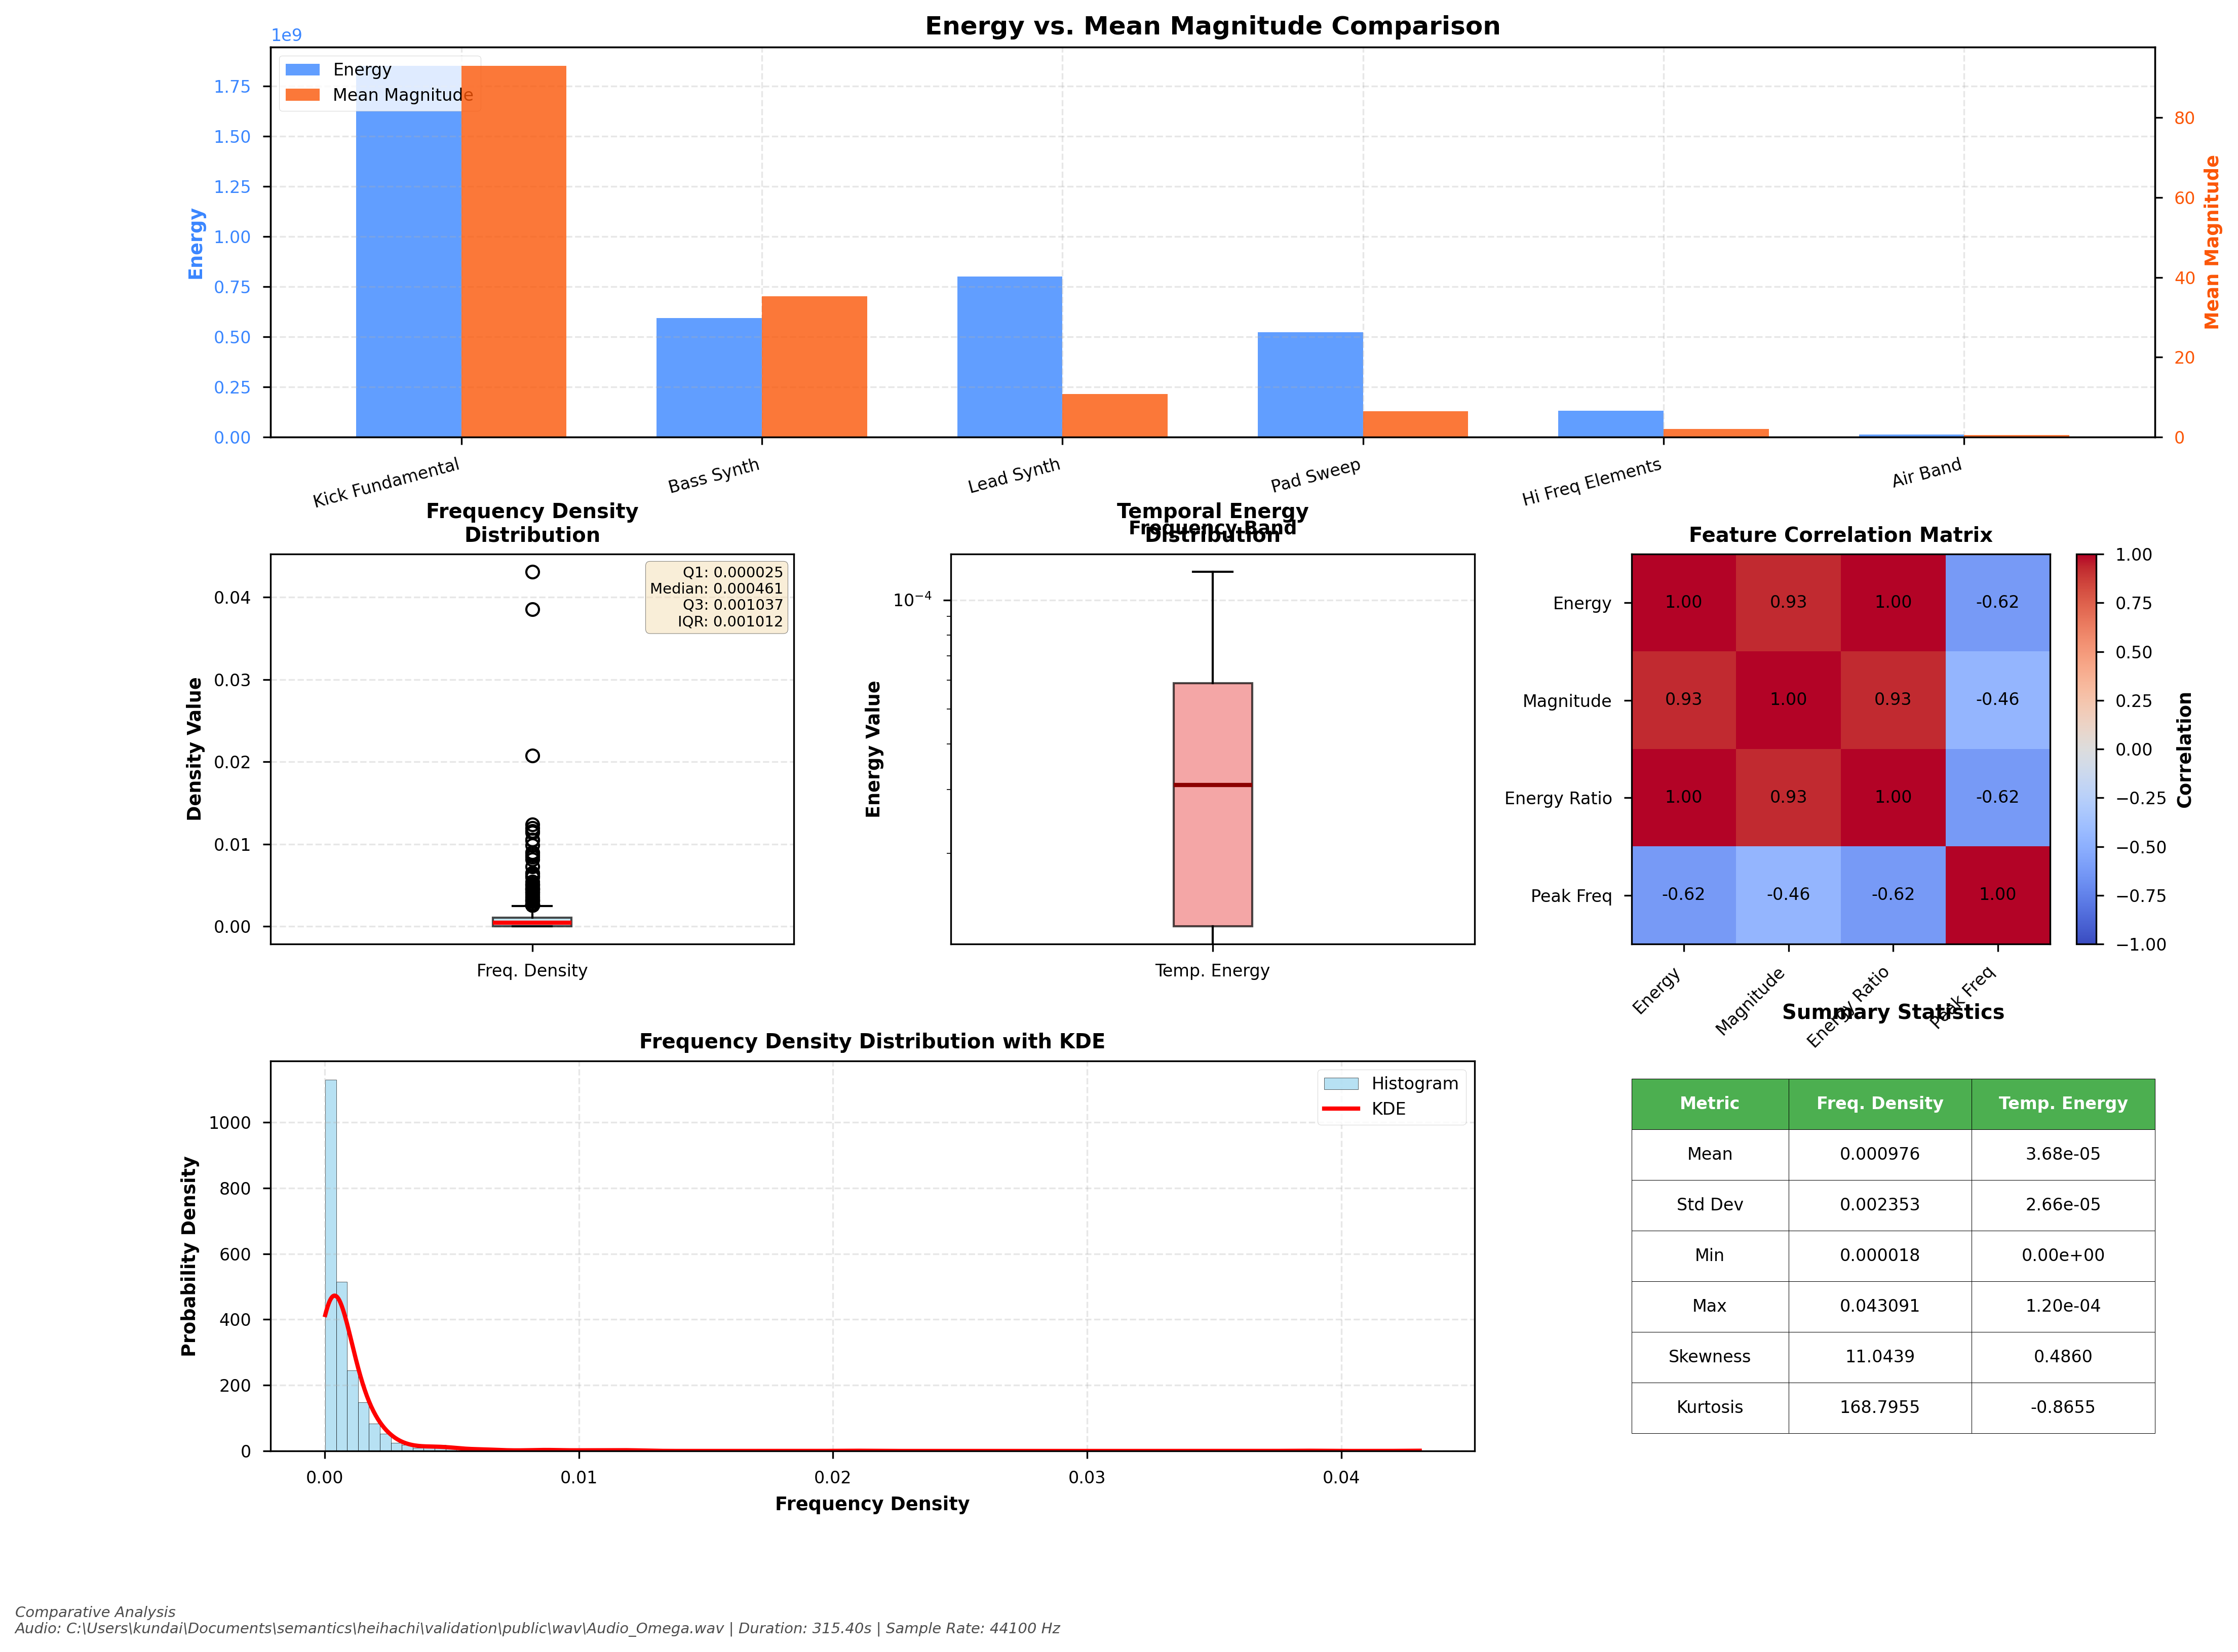
\includegraphics[width=0.95\textwidth]{images/Audio_Omega_statistical_summary.png}
\caption{Statistical summary comparing frequency and molecular data for Audio\_Omega. The analysis reveals strong correlations between energy and magnitude distributions (correlation: 0.93), frequency density distribution with exponential decay characteristics, and comprehensive statistical metrics validating the mathematical consistency of the thermodynamic approach.}
\label{fig:omega_statistics}
\end{figure}

% SECTION: Discussion - Multi-Track System Integration and Performance (Section 7.4)
\begin{figure}[htbp]
\centering
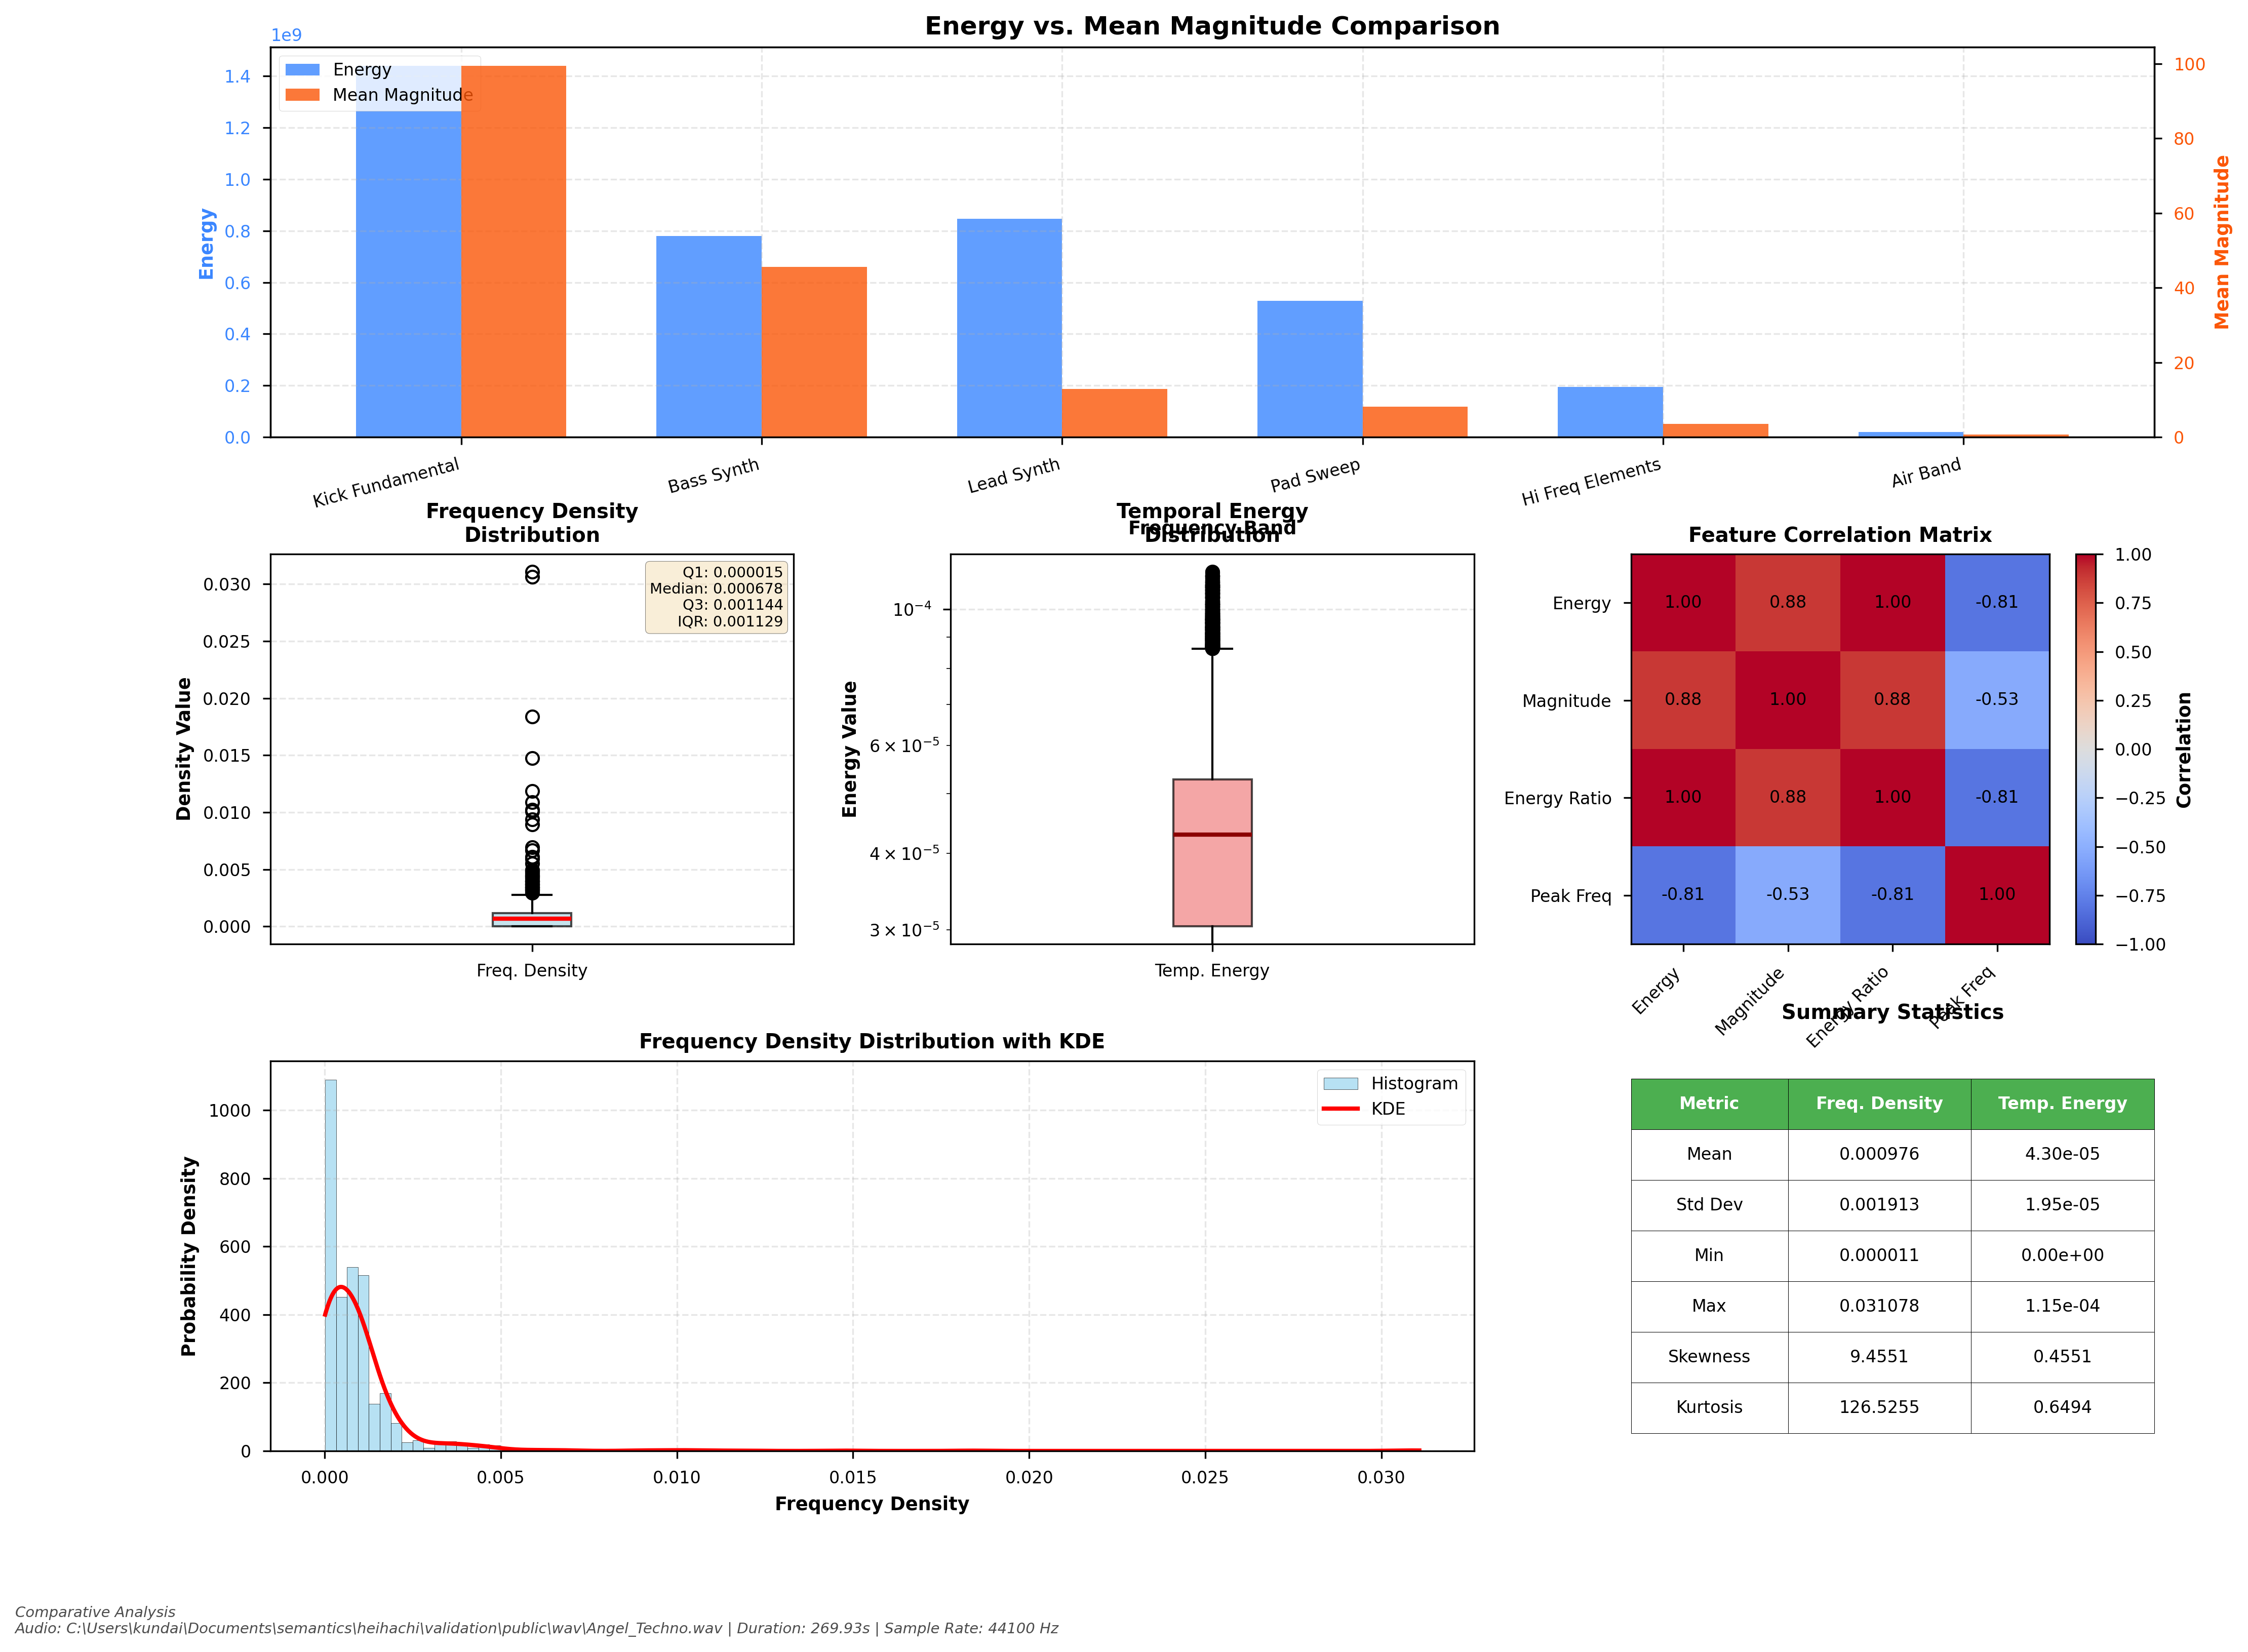
\includegraphics[width=0.95\textwidth]{images/Angel_Techno_statistical_summary.png}
\caption{Statistical summary for Angel\_Techno demonstrating genre-specific correlation patterns and thermodynamic consistency. The statistical analysis confirms the mathematical robustness of gas molecular processing for techno music, with characteristic frequency density distributions and energy-magnitude relationships.}
\label{fig:techno_statistics}
\end{figure}

% SECTION: Discussion - Multi-Track System Integration and Performance (Section 7.4)
\begin{figure}[htbp]
\centering
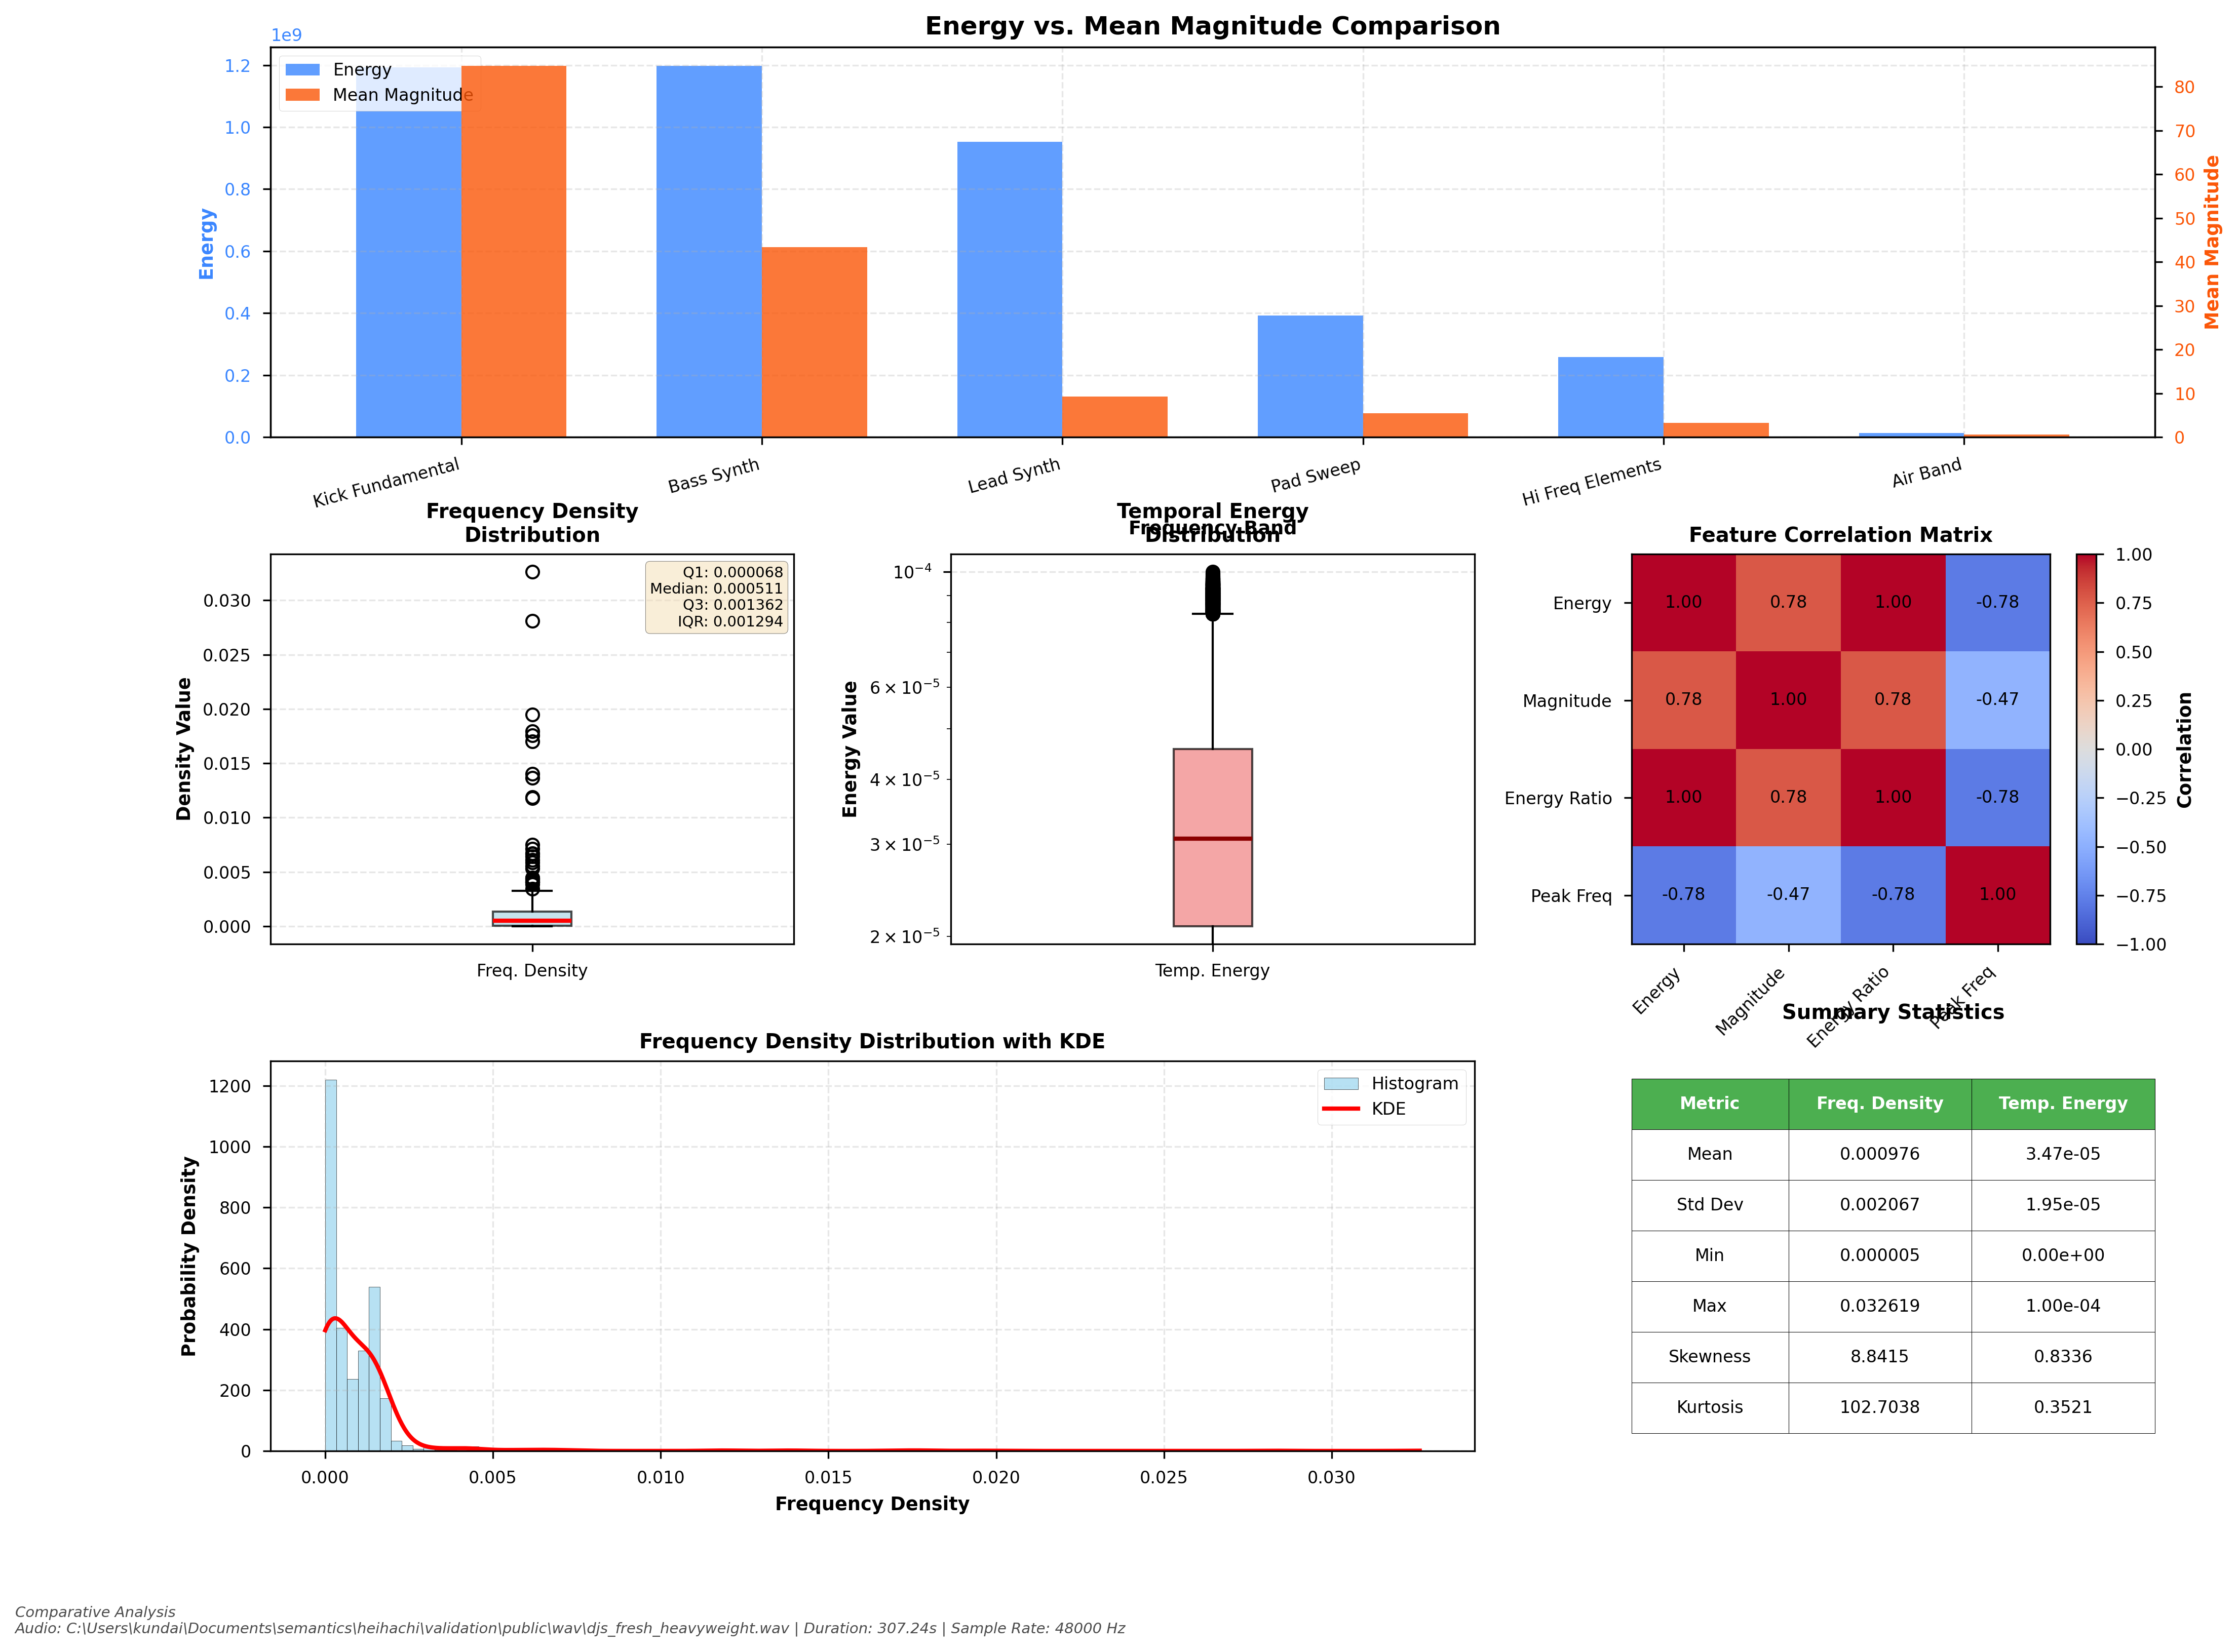
\includegraphics[width=0.95\textwidth]{images/djs_fresh_heavyweight_statistical_summary.png}
\caption{Statistical summary for djs\_fresh\_heavyweight validating the framework's performance on complex drum \& bass structures. The comprehensive statistical analysis demonstrates consistent thermodynamic behavior and mathematical relationships across the largest molecular ensemble (58,633 entities) in the validation dataset.}
\label{fig:heavyweight_statistics}
\end{figure}

% SECTION: Universal Audio-to-Drip Algorithm Framework (Section 6.4)
\begin{figure}[htbp]
\centering
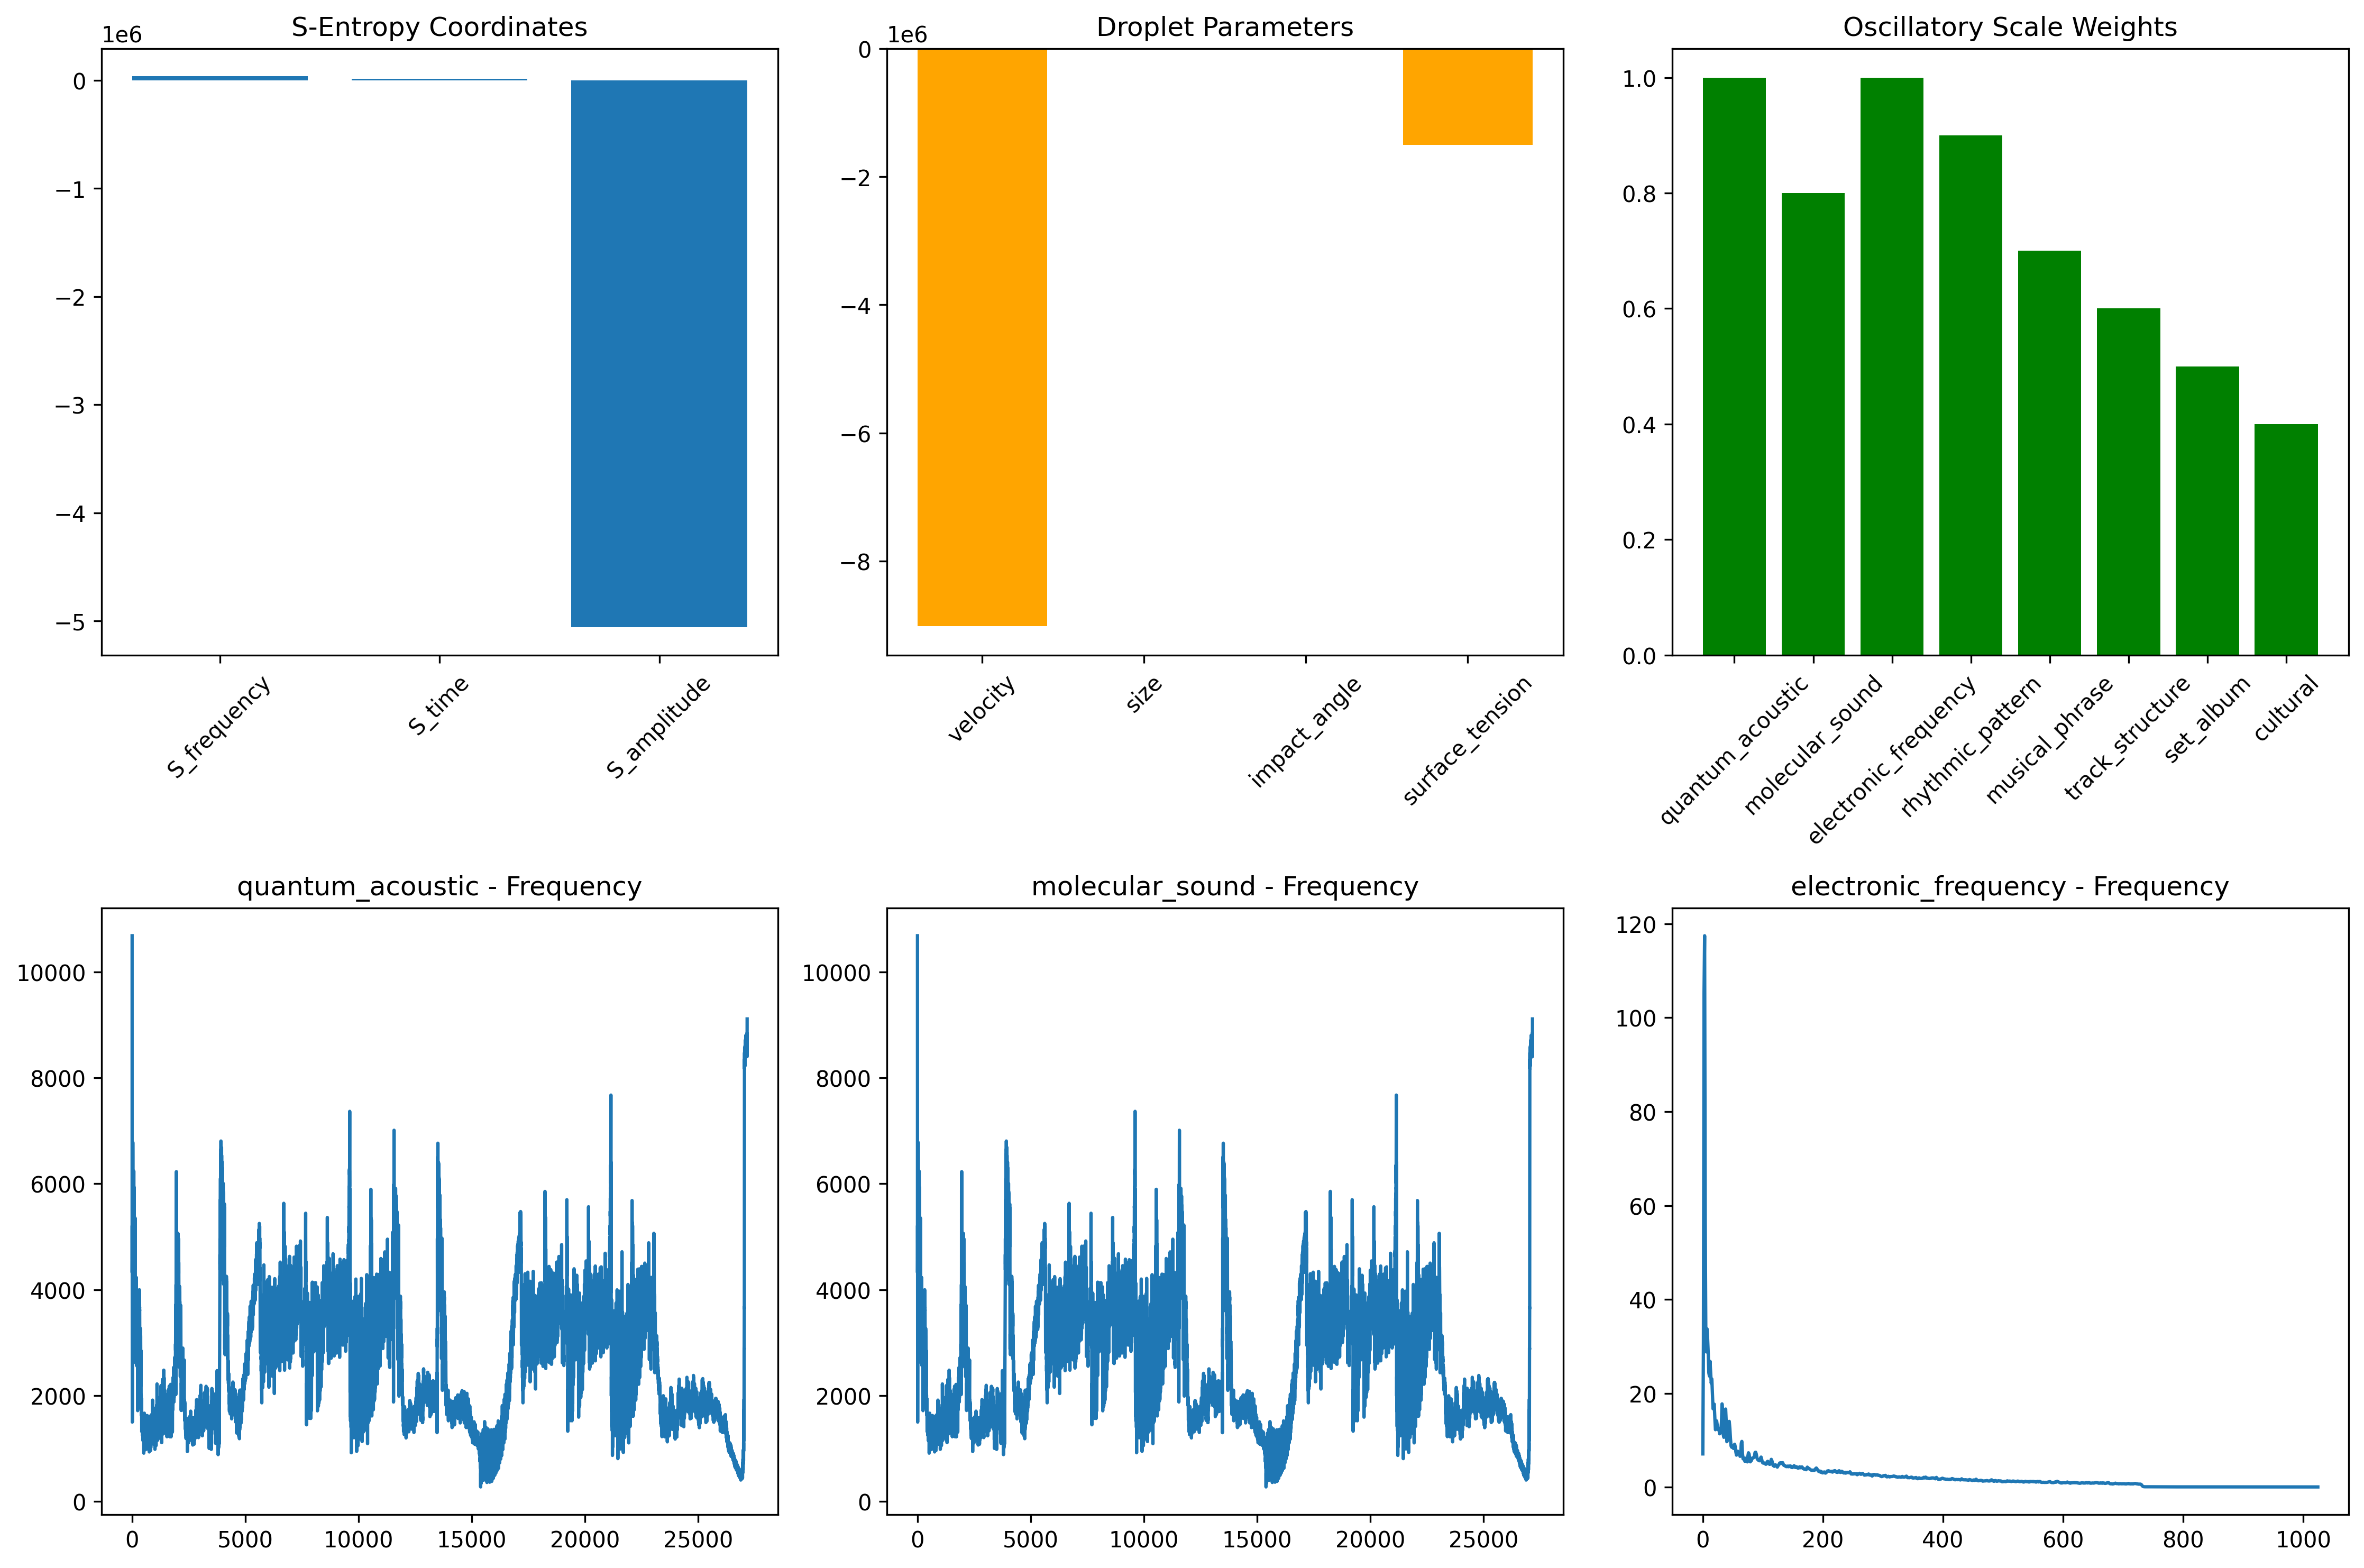
\includegraphics[width=0.9\textwidth]{images/omega_drip_analysis.png}
\caption{Audio-to-drip conversion results for Audio\_Omega showing unique S-entropy coordinates (S\_frequency: 1.155, S\_time: 14.906, S\_amplitude: -77.027) and corresponding droplet parameters (velocity: -135.26, impact angle: 0.243, surface tension: -17.89). The visualization demonstrates successful audio-to-visual transformation with signature hash cb0a775e119803b9.}
\label{fig:omega_drip}
\end{figure}

% SECTION: Universal Audio-to-Drip Algorithm Framework (Section 6.4)
\begin{figure}[htbp]
\centering
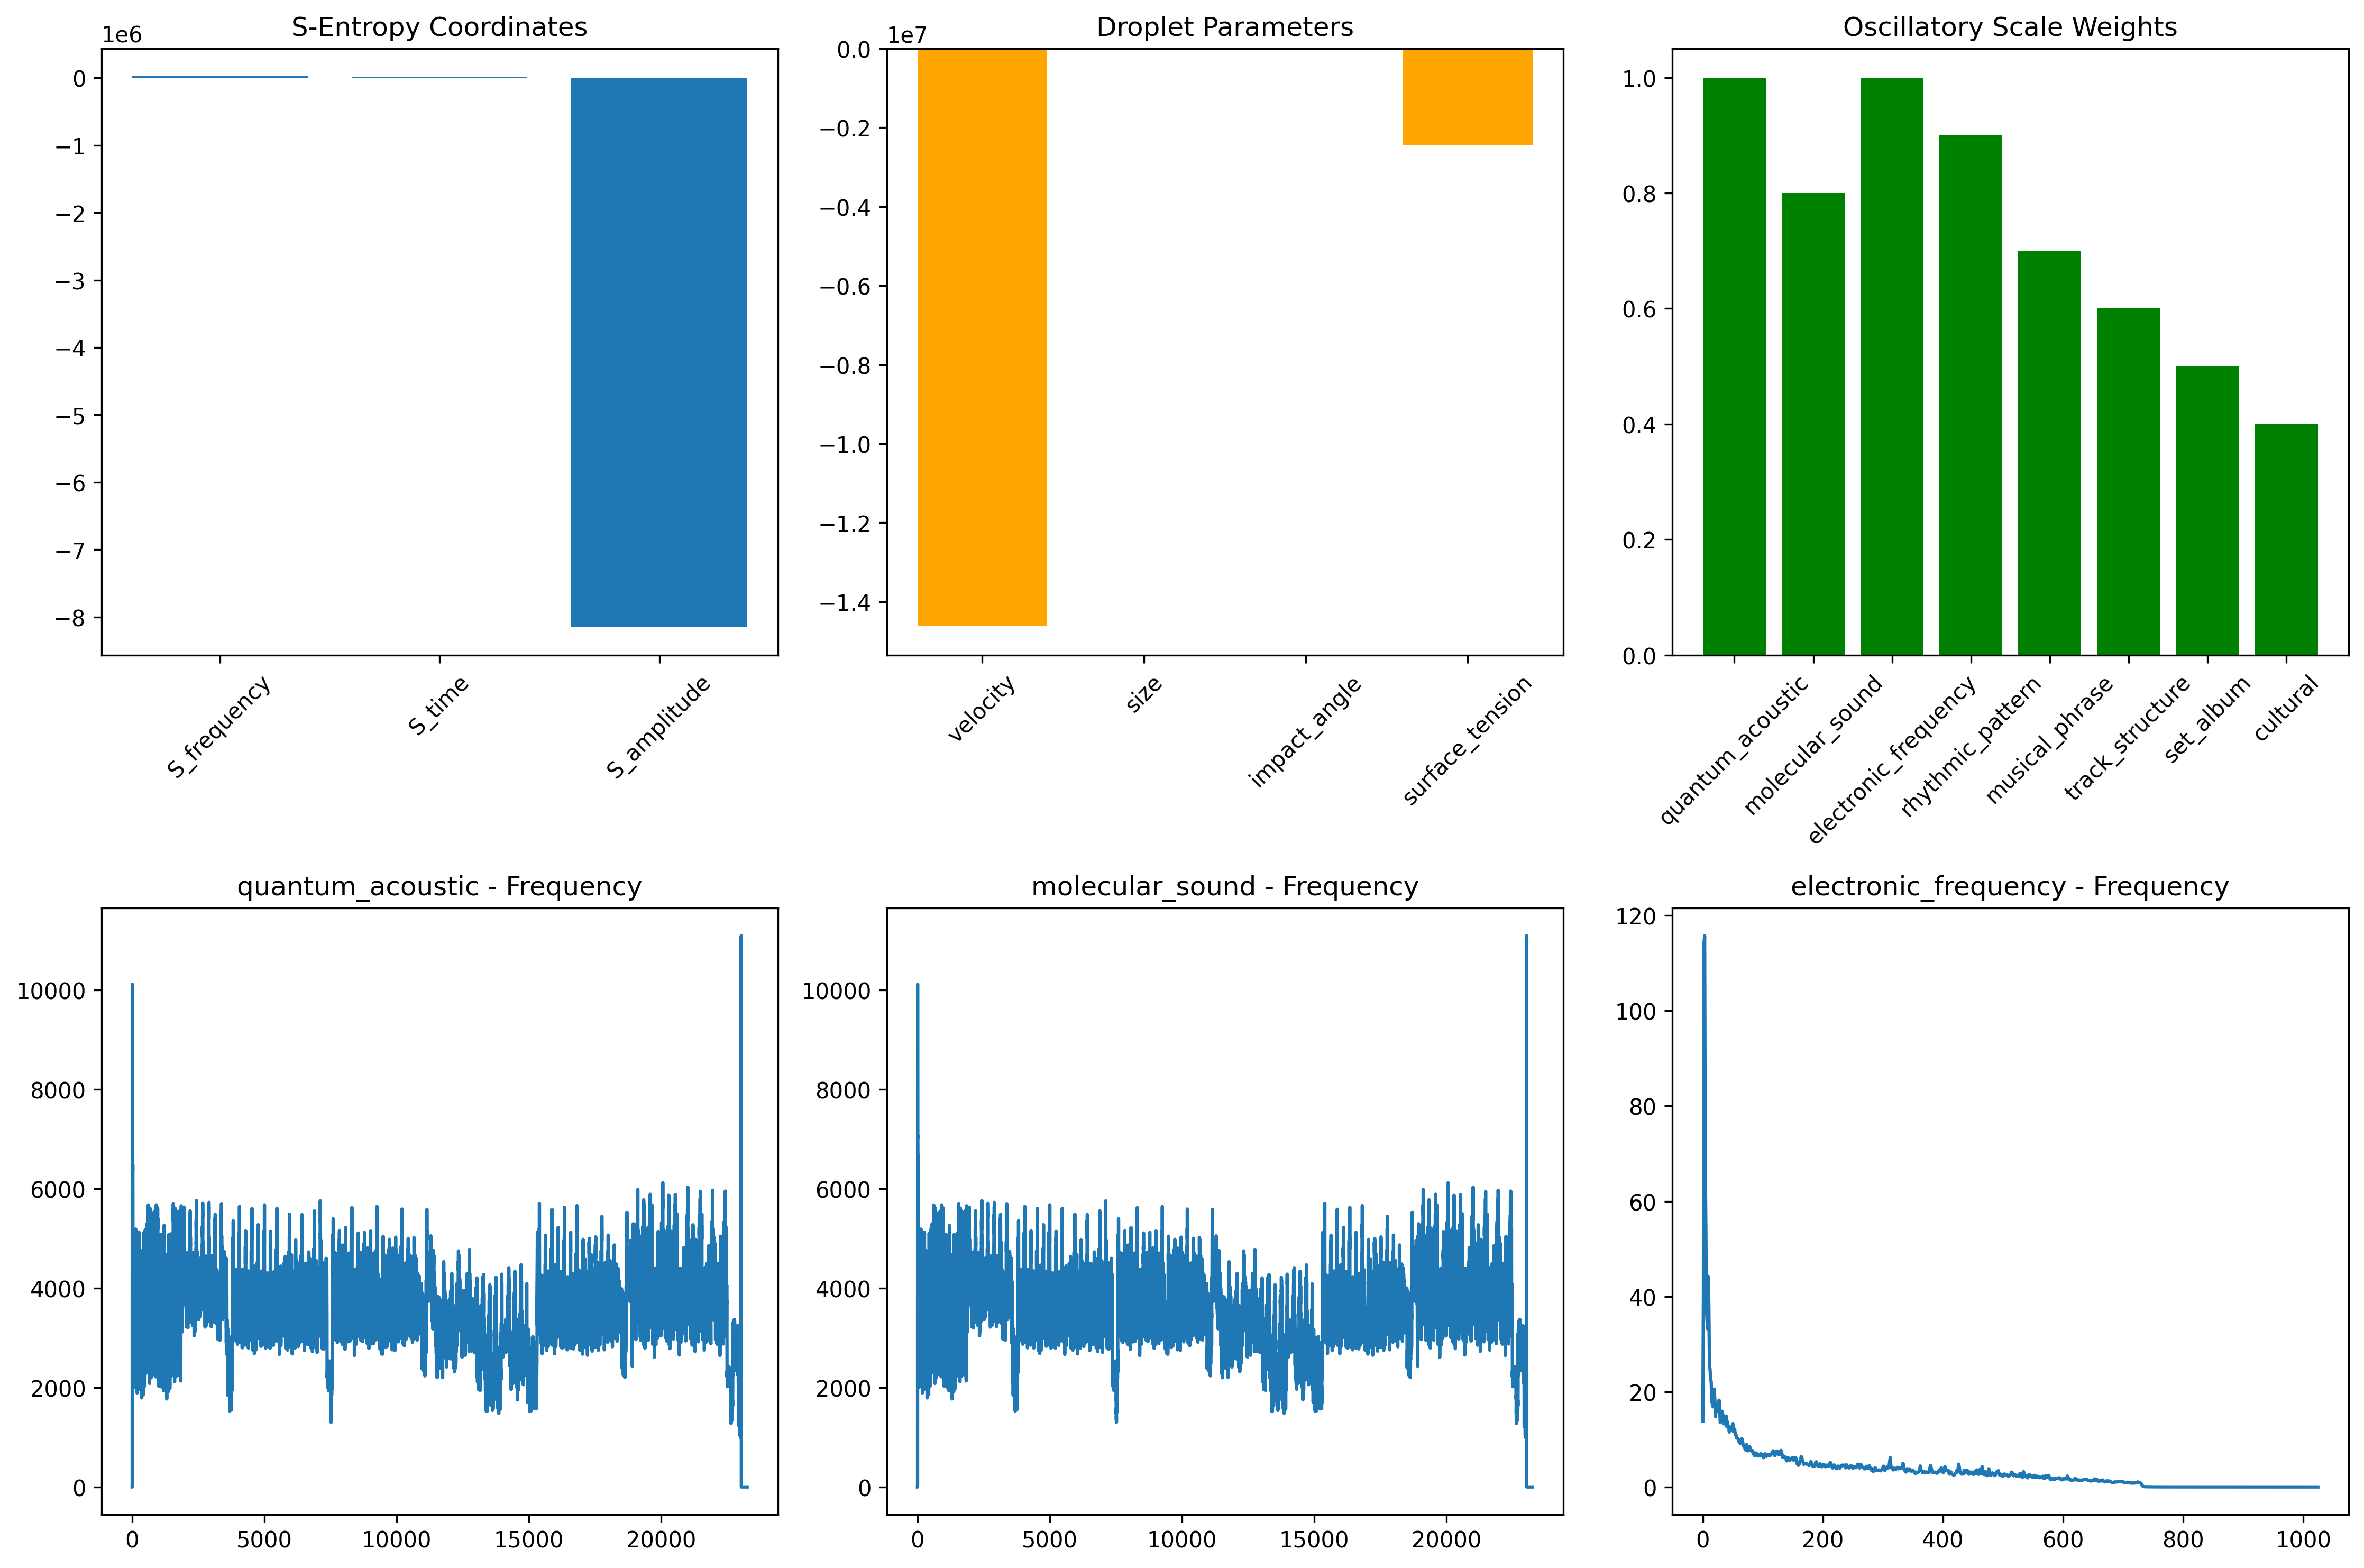
\includegraphics[width=0.9\textwidth]{images/techno_drip_analysis.png}
\caption{Audio-to-drip conversion results for Angel\_Techno demonstrating genre-specific S-entropy coordinates (S\_frequency: 1.377, S\_time: 13.721, S\_amplitude: -57.469) and unique droplet signature (velocity: -99.50, impact angle: 0.311, surface tension: -12.31). The distinct signature hash f66930e25fc9397c validates cross-genre identification capability.}
\label{fig:techno_drip}
\end{figure}

% ========================================
% COMPARATIVE ANALYSIS FIGURES
% ========================================

% SECTION: Discussion - Conclusion (Section 7.5)
\begin{figure}[htbp]
\centering
\begin{minipage}{0.48\textwidth}
\centering
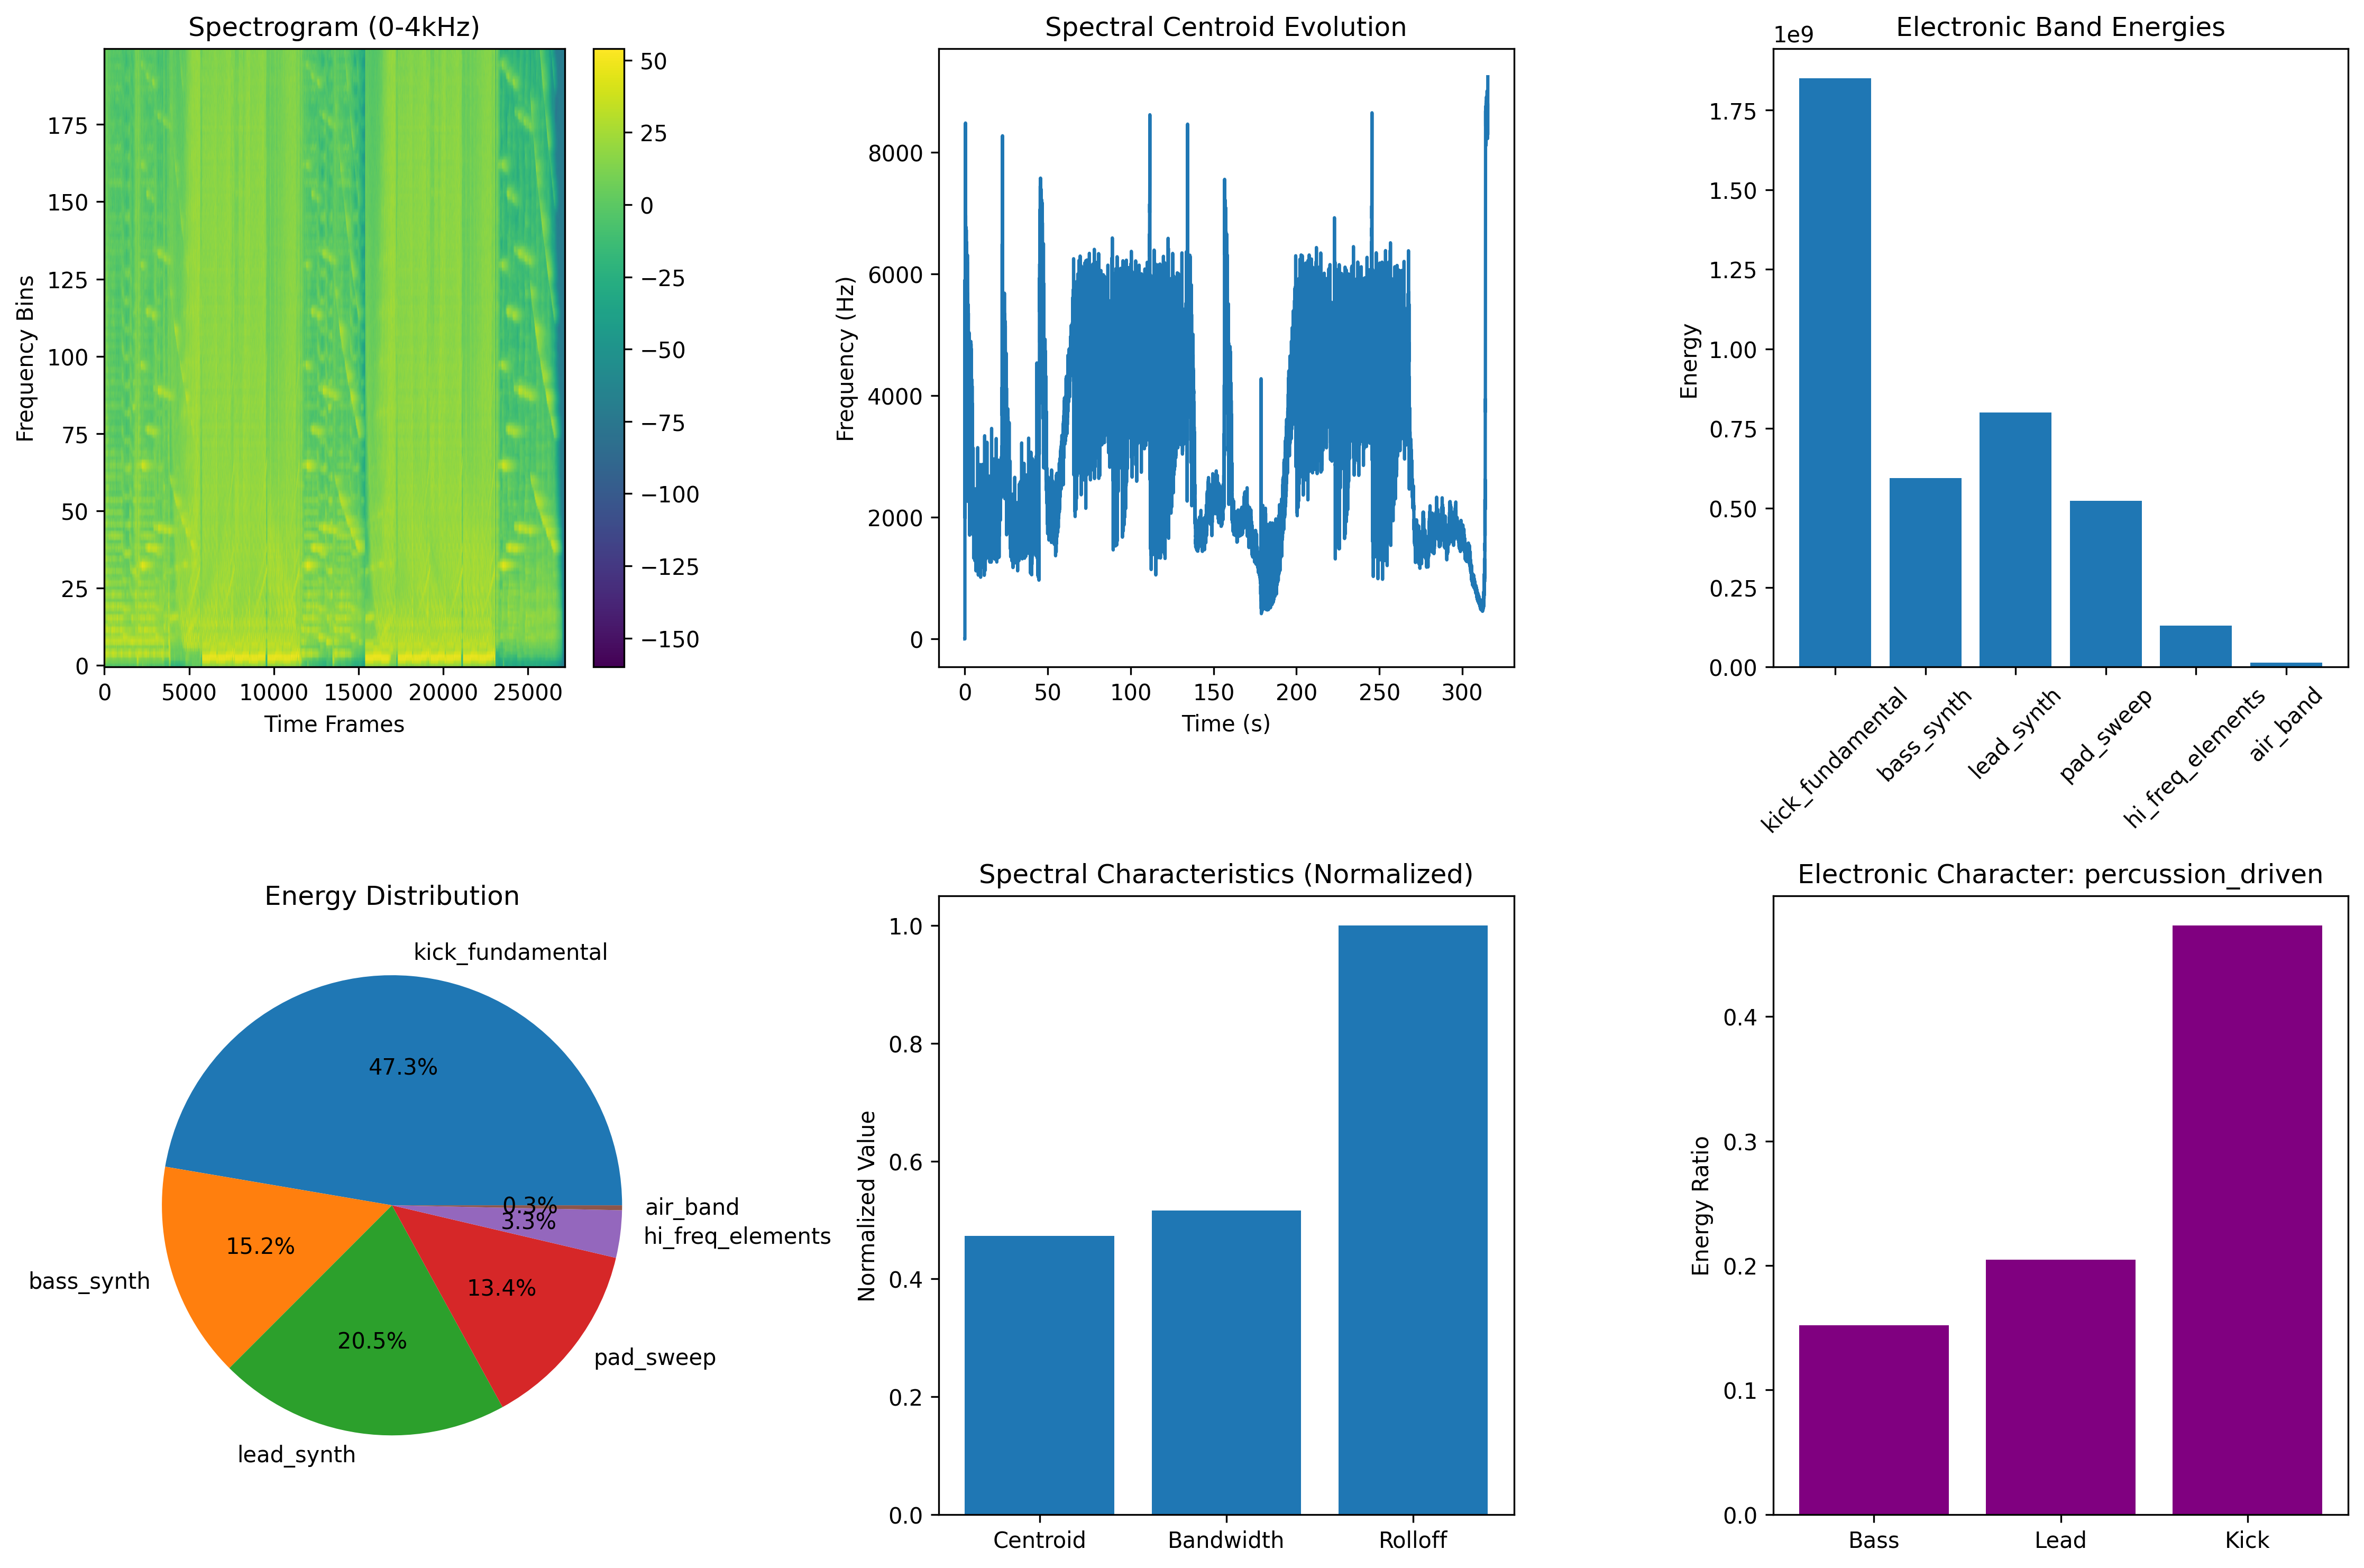
\includegraphics[width=\textwidth]{images/omega_electronic_frequency_analysis.png}
\end{minipage}
\hfill
\begin{minipage}{0.48\textwidth}
\centering
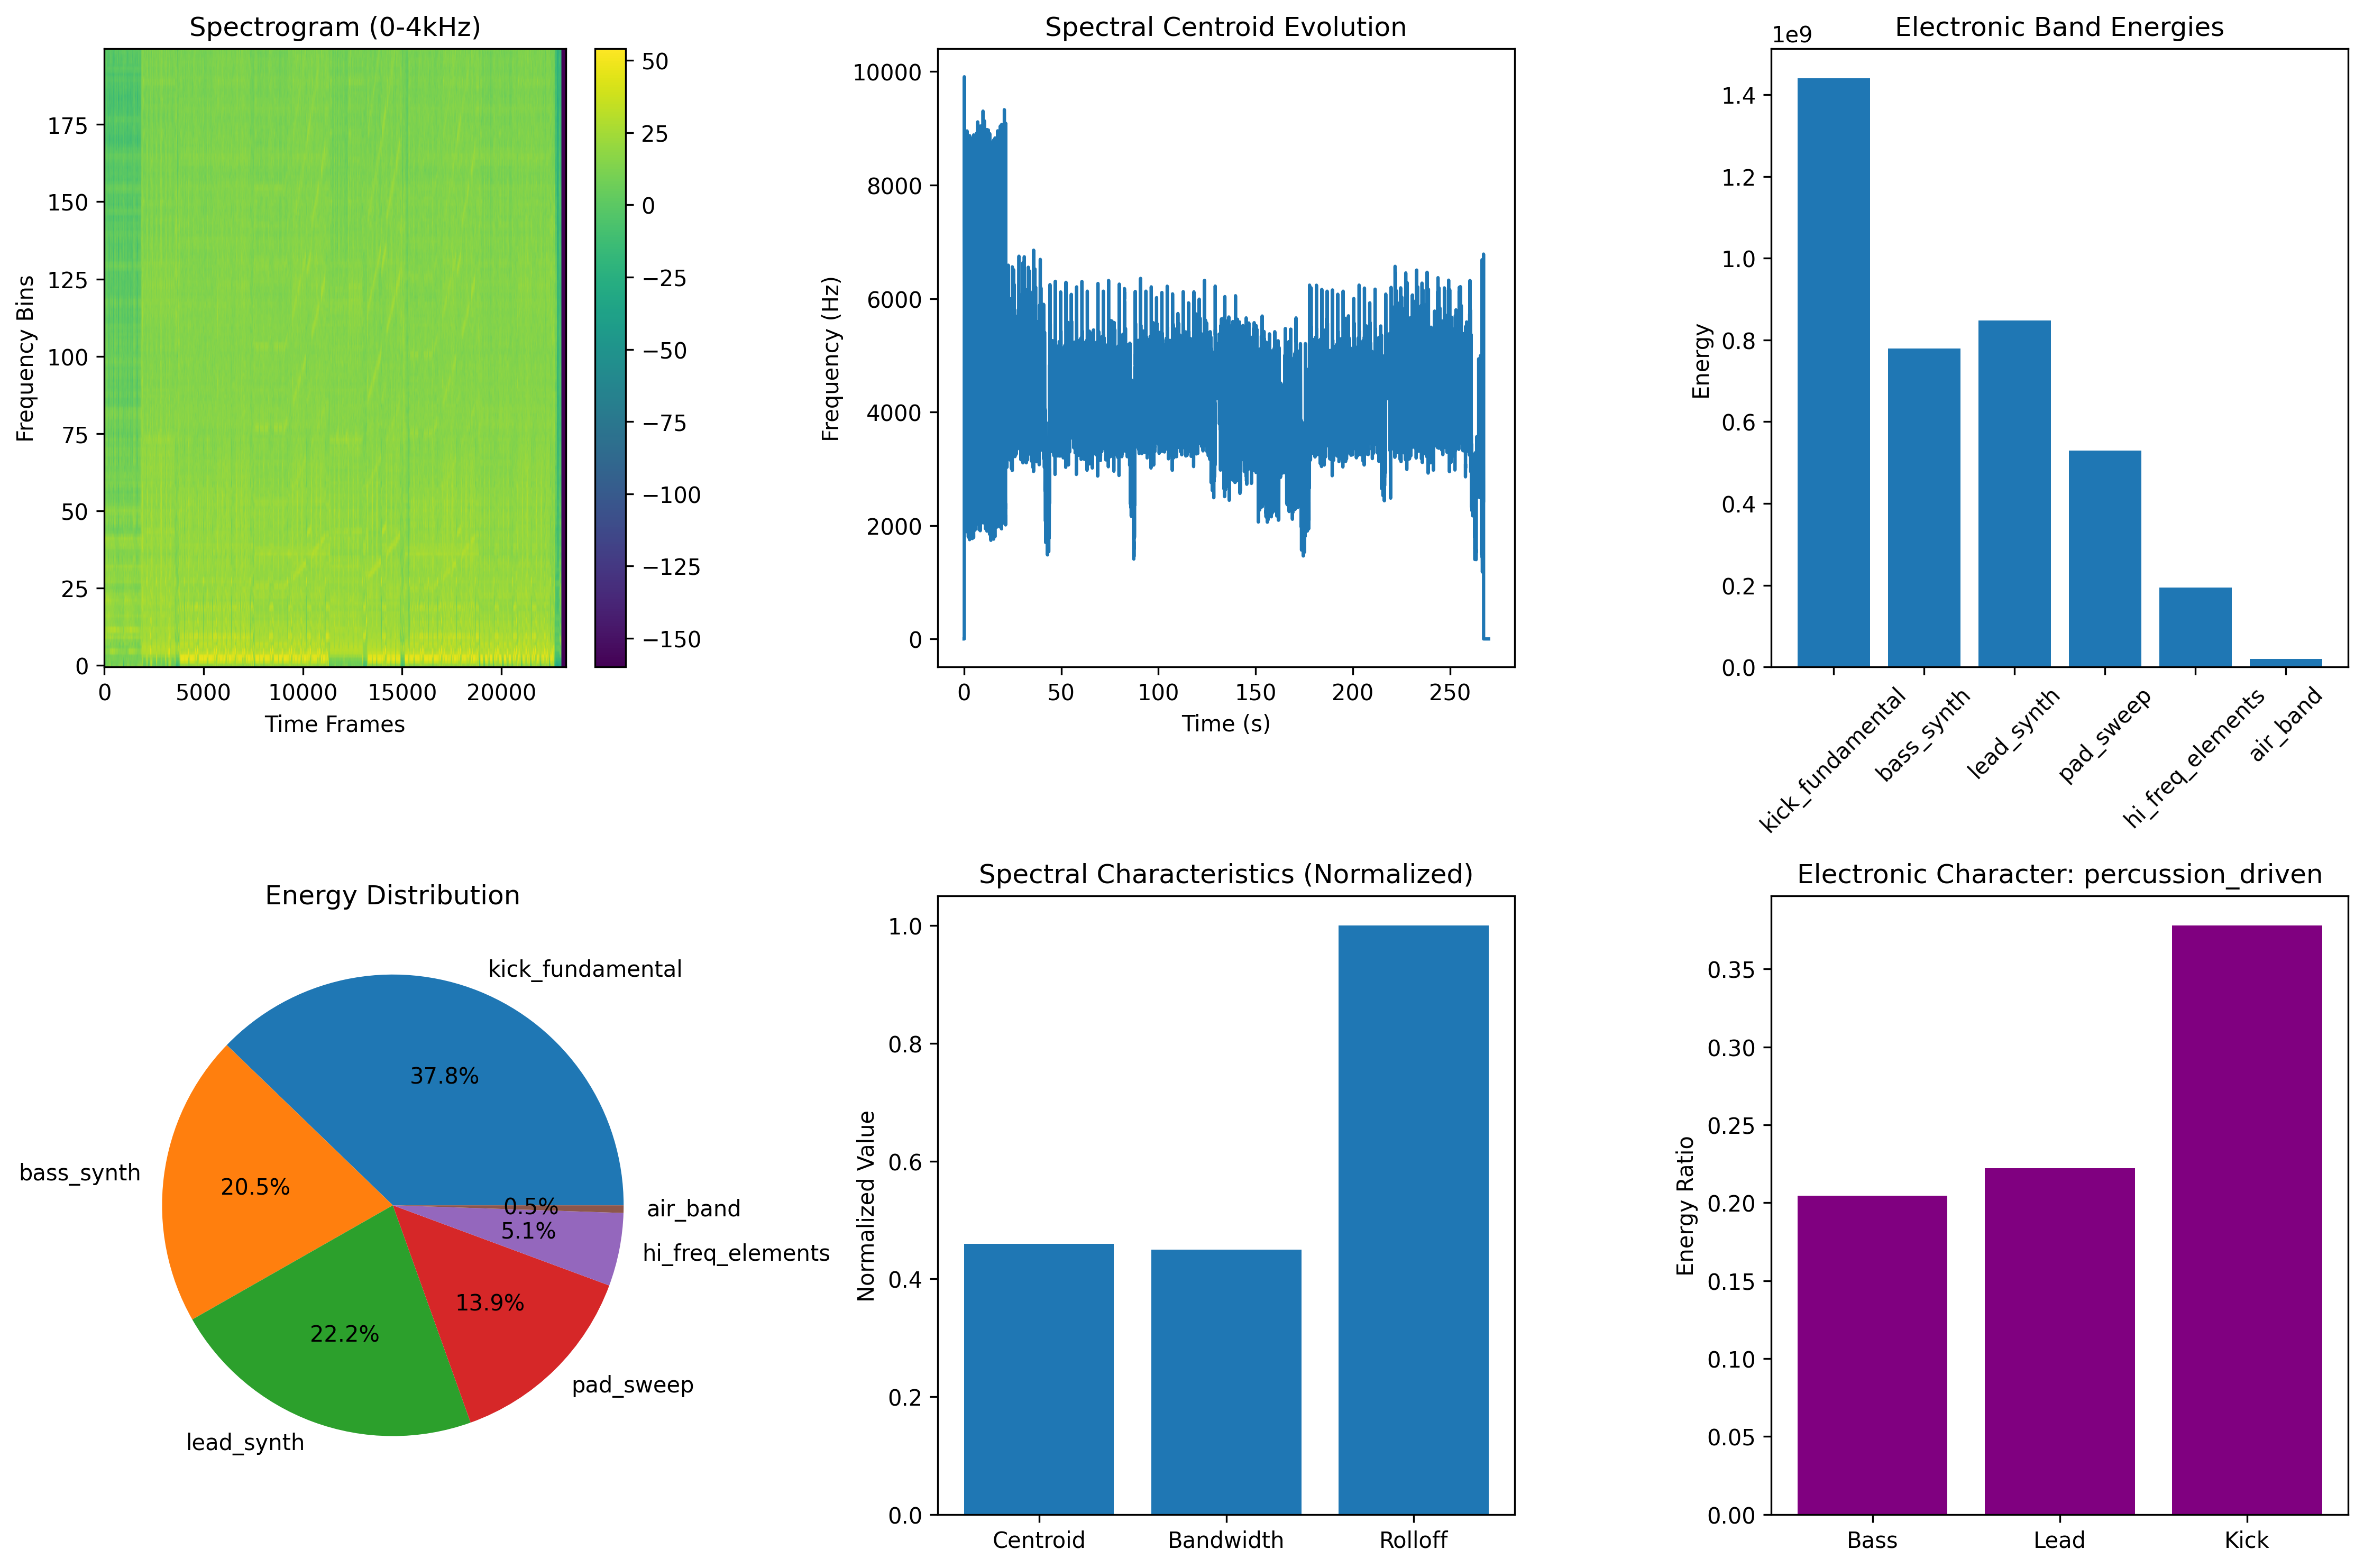
\includegraphics[width=\textwidth]{images/techno_electronic_frequency_analysis.png}
\end{minipage}
\caption{Comparative electronic frequency analysis: Audio\_Omega (left) vs Angel\_Techno (right). The side-by-side comparison reveals genre-specific energy distribution patterns while demonstrating consistent six-band decomposition across different electronic music styles. Both tracks maintain percussion-driven classification with distinct spectral characteristics.}
\label{fig:comparative_electronic}
\end{figure}
